\documentclass[edeposit,fullpage]{uiucthesis2009}

% Import all packages in Copernicus.
\usepackage[normalem]{ulem}
\usepackage[T1]{fontenc}
\usepackage{textcomp}
\usepackage[utf8]{inputenc}
\usepackage[english]{babel}
\usepackage{array}
\usepackage{tabularx}
\usepackage{graphicx}
\usepackage{overpic}
\usepackage{color}
\usepackage{amssymb}
\usepackage[intlimits,fleqn,tbtags]{amsmath}
\usepackage{amsthm}
\usepackage{url}\urlstyle{same}
\usepackage{accents}
\usepackage{cancel}
\usepackage{multirow}
\usepackage{supertabular}
\usepackage{algorithmic}
\usepackage{float}
\usepackage{algorithm}
\usepackage{caption}
%\usepackage{subfig}
%\usepackage{subfloat}
\usepackage[authoryear,round]{natbib}
\usepackage{rotating}
\usepackage[mathlines,modulo]{lineno}
\usepackage{times}
\usepackage{tikz}
\usepackage{subcaption}  %package for acp paper
\usepackage[version=4]{mhchem} % package for jgr paper
%\usepackage{chemformula}
\usepackage{threeparttable} %% package for jgr paper
\usepackage{booktabs}
\usepackage{soul}
\usetikzlibrary{shapes,arrows,chains}

%
\renewcommand{\topfraction}{0.9}	% max fraction of floats at top
\renewcommand{\bottomfraction}{0.8}	% max fraction of floats at bottom

% TODO commands
\newcommand{\jctodo}[1]{{\color{red} #1}}
\newcommand{\jcedits}[1]{{\color{blue} #1}}

% Graphics path
\graphicspath{{./graphics/}}

\pdfinfo{
   /Author (Yu Yao)
   /Title  (Particle-resolved aerosol modeling on the
regional scale -- Insights into importance of capturing
aerosol mixing state)
%   /CreationDate (D:20040502195600)
}

% Custom settings
\renewcommand\thealgorithm{\thechapter.\arabic{algorithm}} 

% Tables
\newcommand\tophline{\hline\noalign{\vspace{1mm}}}
\newcommand\middlehline{\noalign{\vspace{1mm}}\hline\noalign{\vspace{1mm}}}
\newcommand\bottomhline{\noalign{\vspace{1mm}}\hline}
\newcommand\hhline{\noalign{\vspace{1mm}}\hline\noalign{\vspace{1mm}}}

% Need the GMD unit command
\DeclareRobustCommand*\unit[1]
 {\ensuremath{%
   {\thinmuskip3mu\relax
    \def\mu{\text{\textmu}}\def~{\,}%
    \ifx\f@series\testbx\mathbf{#1}\else\mathrm{#1}\fi}}}

    
\newcommand{\kMax}{K_{\textnormal{up}}}
\newcommand{\kMin}{K_{\textnormal{min}}}
\newcommand{\kOver}{K_{\textnormal{over}}}
\newtheorem{theorem}{Theorem}[chapter]
\newtheorem{corollary}[theorem]{Corollary}

% Adjust the length of the table of contents
% List everything (subsubsections)
%\setcounter{tocdepth}{3}
% Chapters and sections only
\setcounter{tocdepth}{1}
\begin{document}

%%%% Title creation
%\nocopyrightpage
\title{Quantifying cloud chemical processes and aerosol optical properties using a particle--resolved model}
\author{Yu Yao}
\department{Atmospheric Sciences}
\phdthesis
\committee{ Professor Nicole Riemer, Chair and Director of Research\\
Professor Sonia Lasher-Trapp \\
Associate Professor Matthew West \\
Dr. Matt Dawson\\}
\maketitle


% Begin front matter
\frontmatter

\begin{abstract}

\end{abstract}

\begin{dedication}
To my family
\end{dedication}

\chapter*{Acknowledgments}


% List of acknowledgements:
%
% Advisors
% Department support, specifically committee.
% Riemer group, specifically Joseph Ching, Laura Fierce.
% CSE fellowship
% DOE ASR grant
% Blue Waters standard acknowledgement

%%%%%%
% Next comes ToC, LoT and LoF
%%%%%%

\tableofcontents
%\listoftables
%\listoffigures

%%%%%%
% Begin the main body
%%%%%%
\mainmatter


%%%%%%%%%%%%%%%%%%%%%%%%%%%%%
%%%%%Chapter 1%%%%%%%%%%%%%%%
%%%%%%%%%%%%%%%%%%%%%%%%%%%%%
\chapter{Introduction and motivation}
\label{chapter1}
Aerosols are solid or liquid particles suspended in air. They recently
received tremendous attention by the public because of the ongoing
Covid-19 pandemic caused by the SARS-Cov-2 virus, which is airborne
and transmitted by aerosols
\citep{prather2020reducing,zhang2020identifying,
  miller2021transmission, greenhalgh2021ten}. However, aerosol
particles have been recognized as an important component of air
pollutants even before the Covid-19 pandemic. The health effects of
aerosol particles, especially those with diameters less than 2.5~$\rm
\mu m$ ($\rm PM_{2.5}$), have been investigated for several decades
\citep{bell2007spatial, fann2012estimating} \textcolor{red}{add an
  early citation here, maybe the six city study by Dockery et al,
  1993}. Around 141\,000 premature deaths in North America due to
cardiopulmonary and lung cancer are associated with $\rm PM_{2.5}$
\citep{anenberg2010estimate}. \textcolor{red}{add some statement about
  deaths worldwide (WHO number)}.

Besides its crucial impacts on health, aerosol particles also impact
weather and climate through interacting with solar radiation and
clouds. Large uncertainties still exist regarding quantifying these
impacts \citep{IPCC_CHAPTER7, seinfeld2016improving, fan2016review,
  bellouin2020bounding}. The interaction between aerosols and climate
manifests itself in two ways. On the one hand, aerosol particles
directly alter the Earth's radiative balance by scattering and
absorbing incoming solar radiation, known as aerosol-radiation
interactions (ari). On the other hand, aerosol indirectly affect
climate by influencing cloud properties, such as droplets number
concentration and cloud life, and this effect is known as
aerosol-cloud interactions (aci). Unlike greenhouse gases, aerosols
typically have a short lifetime of only several days, and their
concentrations and properties vary strongly in space and time, causing
the interactions to have the large uncertainties in our predictions of
the future climate.

This dissertation focuses on two specific aspects within the large
topic of aerosol climate effects. The first is to quantify the changes
that aerosol particles experience as a result of aqueous phase
chemistry within clouds. The second is to quantify the error in
aerosol optical properties that is incurred by simplified aerosol
representations, common in current chemical transport models. We
approach both topics from a particle-resolved modeling
perspective. This chapter provides background about aerosol
properties, aerosol climate forcing, aerosol mixing state, mixing
state evolution, model representation for aerosol and aqueous
processes, and formulates the research questions of this work.

\section{Aerosol properties}
\label{cha1-1:aerosol-defi}
%Definition of aerosol particles.
Aerosol particles can be directly emitted from a variety of sources
(primary aerosol) , or formed in the atmosphere from gas precursors
(secondary aerosol). The major components of particles are inorganic
species, carbonaceous species, sea salt and mineral dust
\textcolor{red}{This list doesn't make sense. Sea salt and mineral
  dust are inorganic species.} These species can originate from
natural or anthropogenic sources, and the formation pathways also
depend on the aerosol type. Sea salt particles are generated over
ocean regions through mechanical processes \textcolor{red}{mechanical
  processes sounds mysterious. Just say wave breaking and bubble
  bursting}. Dust is another primary particle type originating mainly
from desert regions and can impact regions at great distances from the
source regions through long-range transport
\citep{van2018mysterious,yu2021observation}. The flux of sea salt and
of mineral dust particles into the atmosphere strongly depends on wind
speed \citep{jaegle2011global, monahan1986model} \textcolor{red}{I
  added mineral dust to this sentence since it applies to both. Add a
  reference for mineral dust}.

Several inorganic aerosol species are secondary in nature, and formed
through either nucleation or gas-to-particle partitioning. For
example, sulfate can form through nucleation of sulfuric acid in the
presence of water vapor \citep{sipila2010role}, and it can also be
produced through oxidation of $\rm SO_2$ by OH in gas phase or $\rm
H_2O_2$ and $\rm O_3$ in the aqueous phase
\citep{shao2019heterogeneous,
  zheng2020multiphase}. \textcolor{red}{add something about nitrate
  and ammonium} Black carbon (BC) and primary organic aerosol (POA)
are usually co-emitted from combustion of fossil fuel and biofuel
\citep{bond2007historical}. The formation of secondary organic aerosol
(SOA) involves partitioning of semivolatile species, oligomerization
\textcolor{red}{can you explain what oligomerization is?} and aqueous
chemistry \citep{zhu2017mechanism, lim2010aqueous, griffin2013sources,
  mcneill2015aqueous}.

It is important to note that particles in the atmosphere are commonly
mixture of different species \textcolor{red}{add a few citations
  here.}. As an example, Figure~\ref{fig:chap1-mixing} shows
transmission electron microscopy (TEM) images of particles collected
in urban Shanghai in 2010.  can Some particles are mixture of two
species (a, b, c), while others are mixture of more than three species
(f, g, h, i).

\begin{figure}
	\centering
	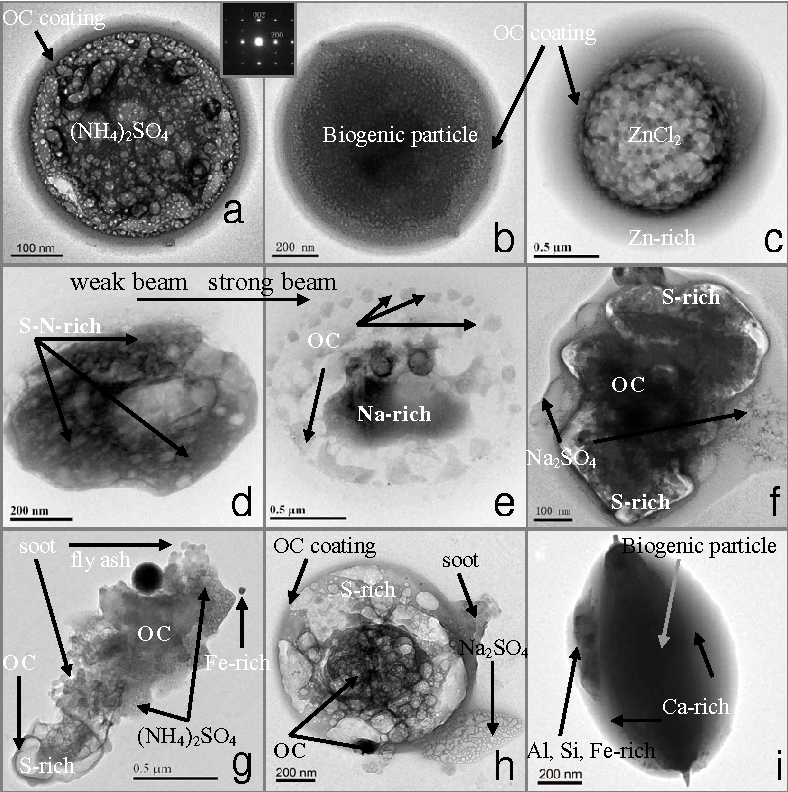
\includegraphics[scale=0.40]{chap1_figs/thesis_chap1_fig2.png}
	\caption{TEM images of carbonaceous particles collected from
          urban Shanghai, adapted from \cite{fu2012morphology}.}
	\label{fig:chap1-mixing}
\end{figure}

%Aerosol particles diameters range from several nanometers to over 10 $\rm \mu m$.  

In addition to exhibiting great diversity with respect to composition,
aerosol particle diameters vary from small molecule clusters of
several nanometers to large particles of several micrometers
\citep{MCMURRY200320}. It is common to represent the aerosol size
distribution by three size ranges, called ``modes'': The nuclei mode
(0.01--0.1 $\rm \mu m$), the accumulation mode (0.1--2 $\rm \mu m$)
and the coarse mode (2--10 $ \rm \mu m$). Nuclei-mode particles are
commonly observed near combustion sources, especially the roadside
atmosphere, and characterized by high number concentration, which
causes efficient coagulation and results in short lifetime of these
particles \citep{fushimi2008atmospheric}. Accumulation-mode particles
contain most of the secondary species, such as sulfate, nitrate and
organics \citep{zhang2005time}, and they can also be produced from the
growth of nuclei-mode particles by coagulation and
condensation. \textcolor{red}{what about the lifetime of accumulation
  mode particles?} As for coarse-mode particles, it is hard to grow
such large particles from accumulation model
\citep{friedlander1991scavenging, lee2005size}. They mostly originate
from natural sources and produced by mechanical processes, and their
lifetime is short in the atmosphere due to rapid gravitational
settling.

\section{Aerosol climate forcing}
\label{cha1-2:aerosl-climate}
Aerosol impact the radiation balance of Earth system through direct
interactions with shortwave and longwave radiation. The globally
averaged direct aerosol effective radiative forcing between 1750 and
2005 \textcolor{red}{2011?} \textcolor{red}{Should use the latest IPCC
  report!} is estimated to be $-0.45$ $\rm W$ $\rm m^{-2}$, as shown
in Fig.~\ref{fig:chap1-aerosol-climate}. Estimation of radiative
forcing relies on the properties of aerosol population, such as size
and chemical components. The large variation of aerosols in different
regions leads to spatial variation of this effect. For example, while
the direct radiative forcing at the top of atmosphere over Africa is
around $-12$ $\rm W$ $\rm m^{-2}$, it can reach $+30$ $\rm W$ $\rm
m^{-2}$ over the polluted Indo-Gangetic Plains
\citep{subba2020recent}.

\begin{figure}
	\centering
	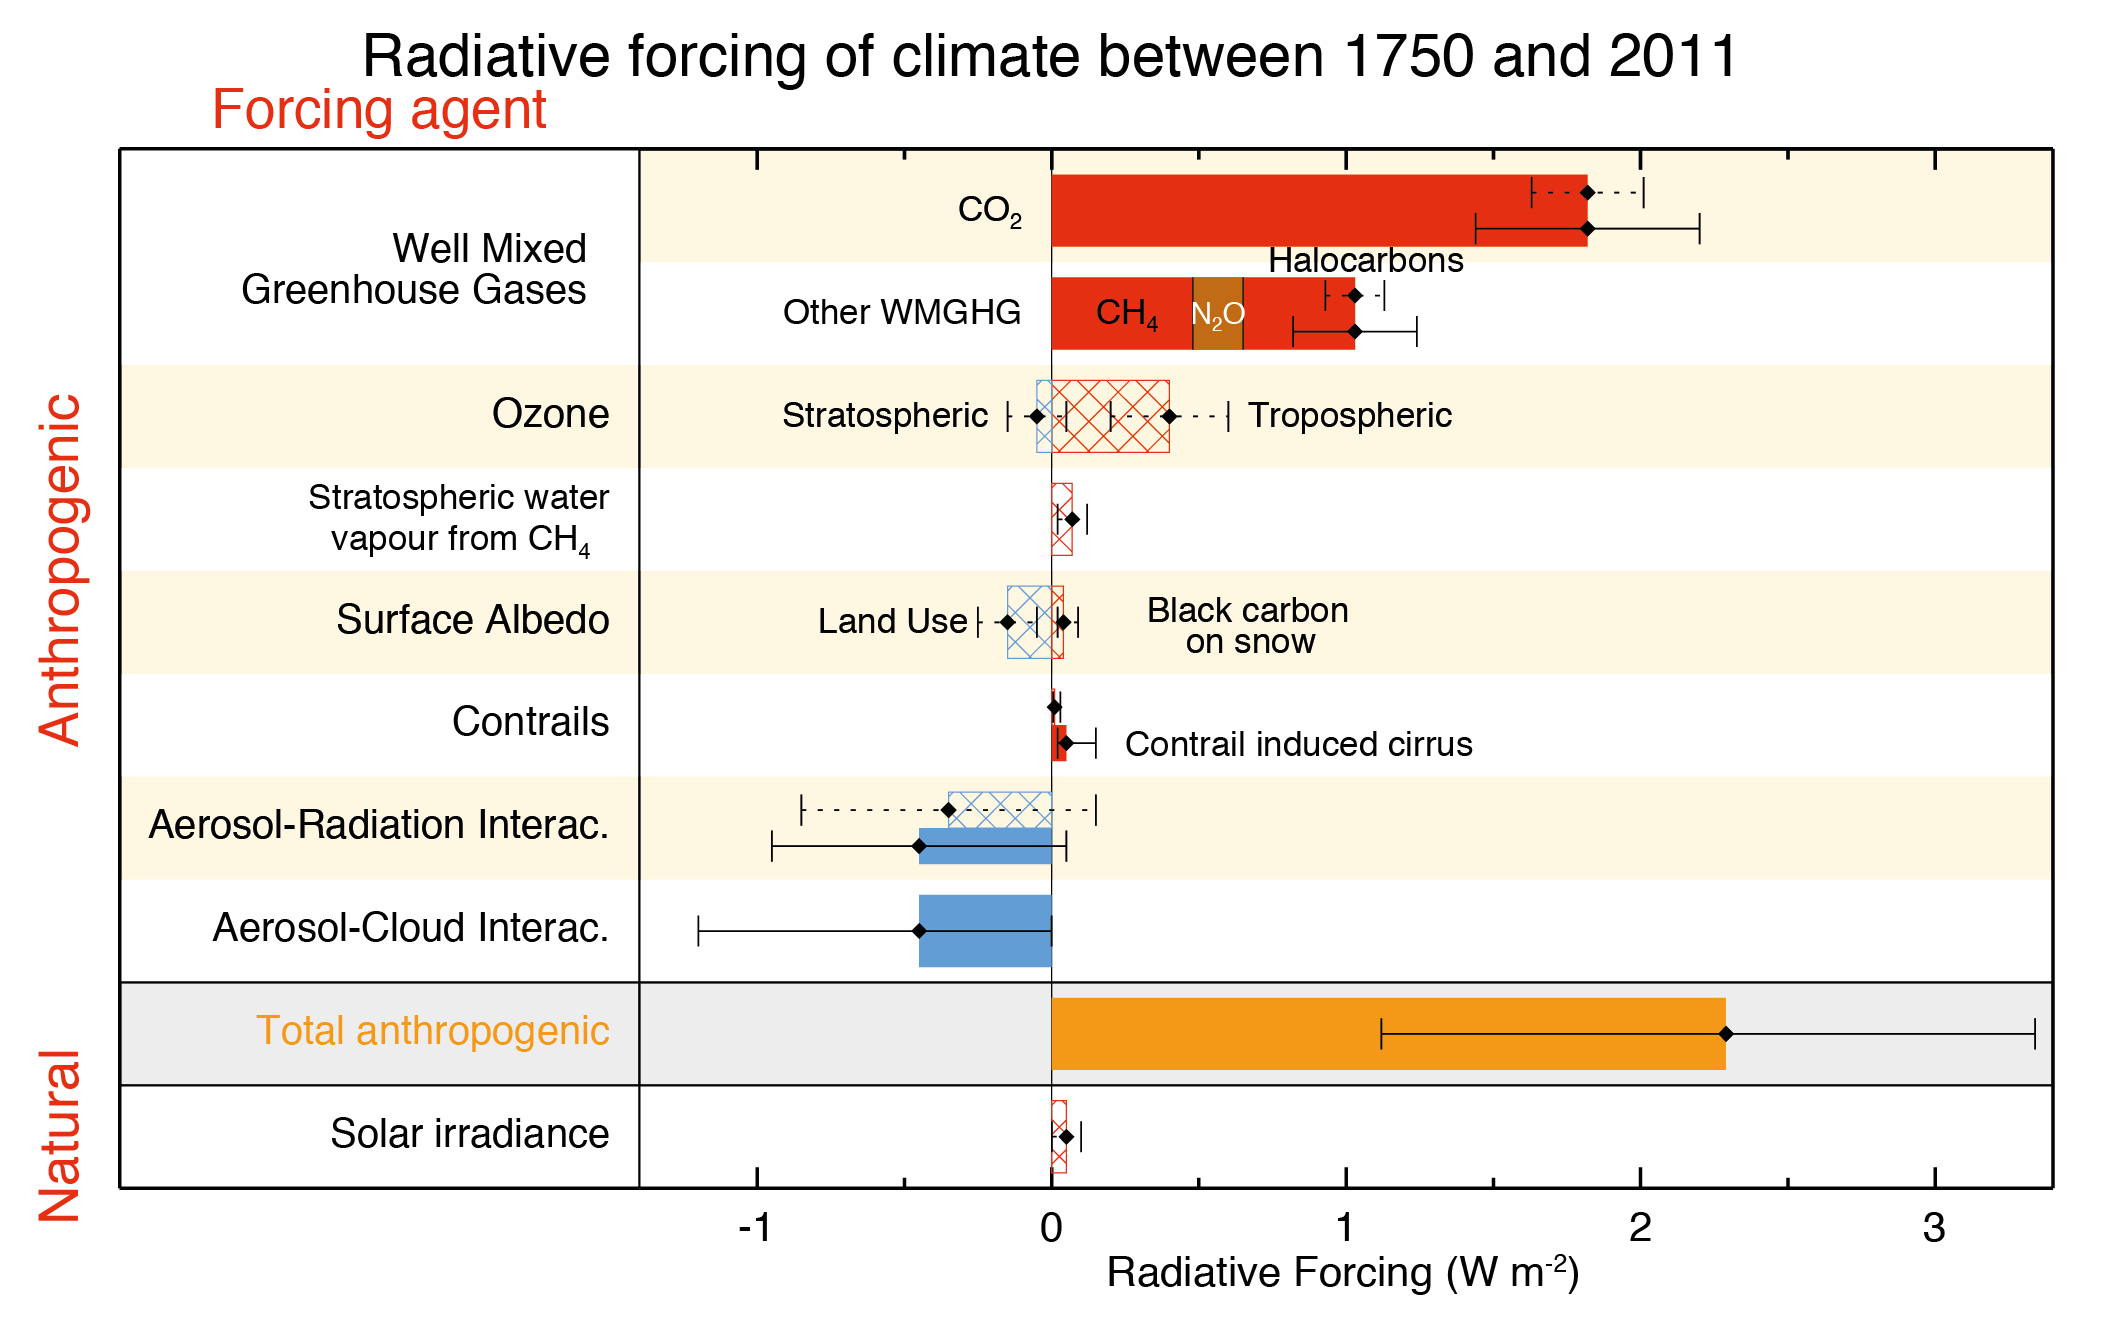
\includegraphics[scale=0.80]{chap1_figs/thesis_chap1_fig1.jpeg}
	\caption{Radiative forcing estimation of different agents between 1750 and 2011, adapted from \cite{IPCC_CHAPTER8}.}
	\label{fig:chap1-aerosol-climate}
\end{figure}

By serving as cloud condensation nuclei, aerosol particles also
indirectly affect climate through interactions with cloud, and the
estimated effective radiative forcing from this interaction is
$-0.45$~\unit{W\;m^{-2}}, similar to the effective direct radiative
forcing (Fig.~\ref{fig:chap1-aerosol-climate}). There are many
processes involved in the interactions, which can be summarized by two
main effects: the cloud albedo and the lifetime
effects. \textcolor{red}{Is this what the bar in figure 1.2 includes?}
Cloud albedo effects, first proposed by \citet{twomey1977influence},
describe the changes of cloud droplet number concentration and surface
area as the number concentration of aerosol particles changes, which
was supported by ambient observations. \citet{kaufman2005effect}, by
analyzing satellite observation over Atlantic ocean, found liquid
clouds coverage in the polluted environment is higher by 0.2$--$0.4
\textcolor{red}{unit?}  than clean environment, and with smaller
droplets. Field observations also confirm that more cloud condensation
nuclei (CCN) generate more cloud droplets with smaller sizes in liquid
clouds
\citep{jia2019distinct,kleinman2012aerosol}. \textcolor{red}{You need
  to be careful here. The cloud albedo effect assumes no changes in
  liquid water content. So the 2005 paper by Kaufman may not be
  relevant.}

The cloud lifetime effect describes the mechanism that the increase of
aerosol number concentration not only results in smaller cloud
droplets but that this inhibits the precipitation development. This
effect is plausible if only the initiation of precipitation is
considered. However, several observation and modeling studies
suggested that it is hard to find clear evidence for this effect due
to the unclear relation between initial cloud droplet size and
evolving precipitation efficiency \citep{stevens2009untangling}
\textcolor{red}{what does unclear mean here?}.
% May do not need to mention this because we are not going to talk about it. 
%The physical understanding of interactions with liquid cloud improves substantially in past decades, but the interactions with ice and mix-phased clouds is still poor constrained. 

As we can see from Fig.~\ref{fig:chap1-aerosol-climate}, large
differences still exist among different models in the magnitude of the
aerosol-related radiative forcing. For the radiative forcing from
aerosol radiation interaction, the estimated 5 to 95\% confidence
interval ranges from $-0.95$ to $+ 0.05$ $\rm W$ $\rm m^{-2}$, while
the range is from $-1.2$ to $0.0$ $\rm W$ $\rm m^{-2}$ for the
radiative forcing due to aerosol-cloud interaction. The sources of the
uncertainty lie in the fact that the processes involved cover a large
range of scales, from particles as small as 10~nm to 1000~km
stratocumulus clouds. Many processes are still not well-understood on
a fundamental level, such as aerosol interaction with mixed-phase and
ice clouds, and simple parameterization schemes are applied to
describe these processes in the models. But even for the processes
that are well-understood on a microscale level, it is challenging to
incorporate all them in a large-scale model
\citep{seinfeld2016improving,bellouin2020bounding}. By interacting
with electromagnetic radiation, and acting as an nuclei for cloud
formation, particles are fundamental for determining radiative forcing
and an accurate description of aerosols can help reduce the model
uncertainty or at least help quantify the uncertainty that is
currently present.

\section{Aerosol mixing state}
The aerosol mixing state refers to the distribution of chemical
species among a particle population and is a helpful framework to
describe aerosols \citep{winkler1973growth}. We distinguish between
two mixing state extremes: the fully internal mixture and the fully
external mixture. As Fig.~\ref{fig:chap1-chi-climate}(a) schematically
shows, a population is considered to be completely internally mixed if
each particle is made up of the same species mixtures, which equals
the bulk composition. For a population with fully external mixture,
each particle only contains one single species. However, in the real
ambient atmosphere, particles rarely fall into any of these two
categories but most likely assume one of many possible intermediate
mixing states. In other words, the number of species and their mass
fractions can differ between particles.

Hygroscopicity and optical properties, which are important factors for
droplets formation and the interaction with radiation, are both
strongly dependint on the chemical species that the particle consists
of. Thus, aerosol population with different mixing states may have
different climate-related properties, as illustrated in
Fig.~\ref{fig:chap1-chi-climate}. Figure~\ref{fig:chap1-chi-climate}(a)
explains this for the example of cloud condensation nuclei
activity. All three populations contain the same amount of ammonium
sulfate and organic matter, but the two species are distributed
differently among the particles. For the internally-mixed population,
each particle has the same amount of ammonium sulfate and organic. For
the externally-mixed population, each particle only contains one
single species. In the real environment, these two species can be
randomly distributed among the particles. If these three populations
are exposed at the same supersaturation (e.g., a supersaturation of
0.3\%), the number of activated particles will be different. All the
particles are activated in the population with internal mixture, while
only 50\% are activated in the externally mixed population. The
activated particles number in real world case are between these two
extremes.

\begin{figure}
	\centering
	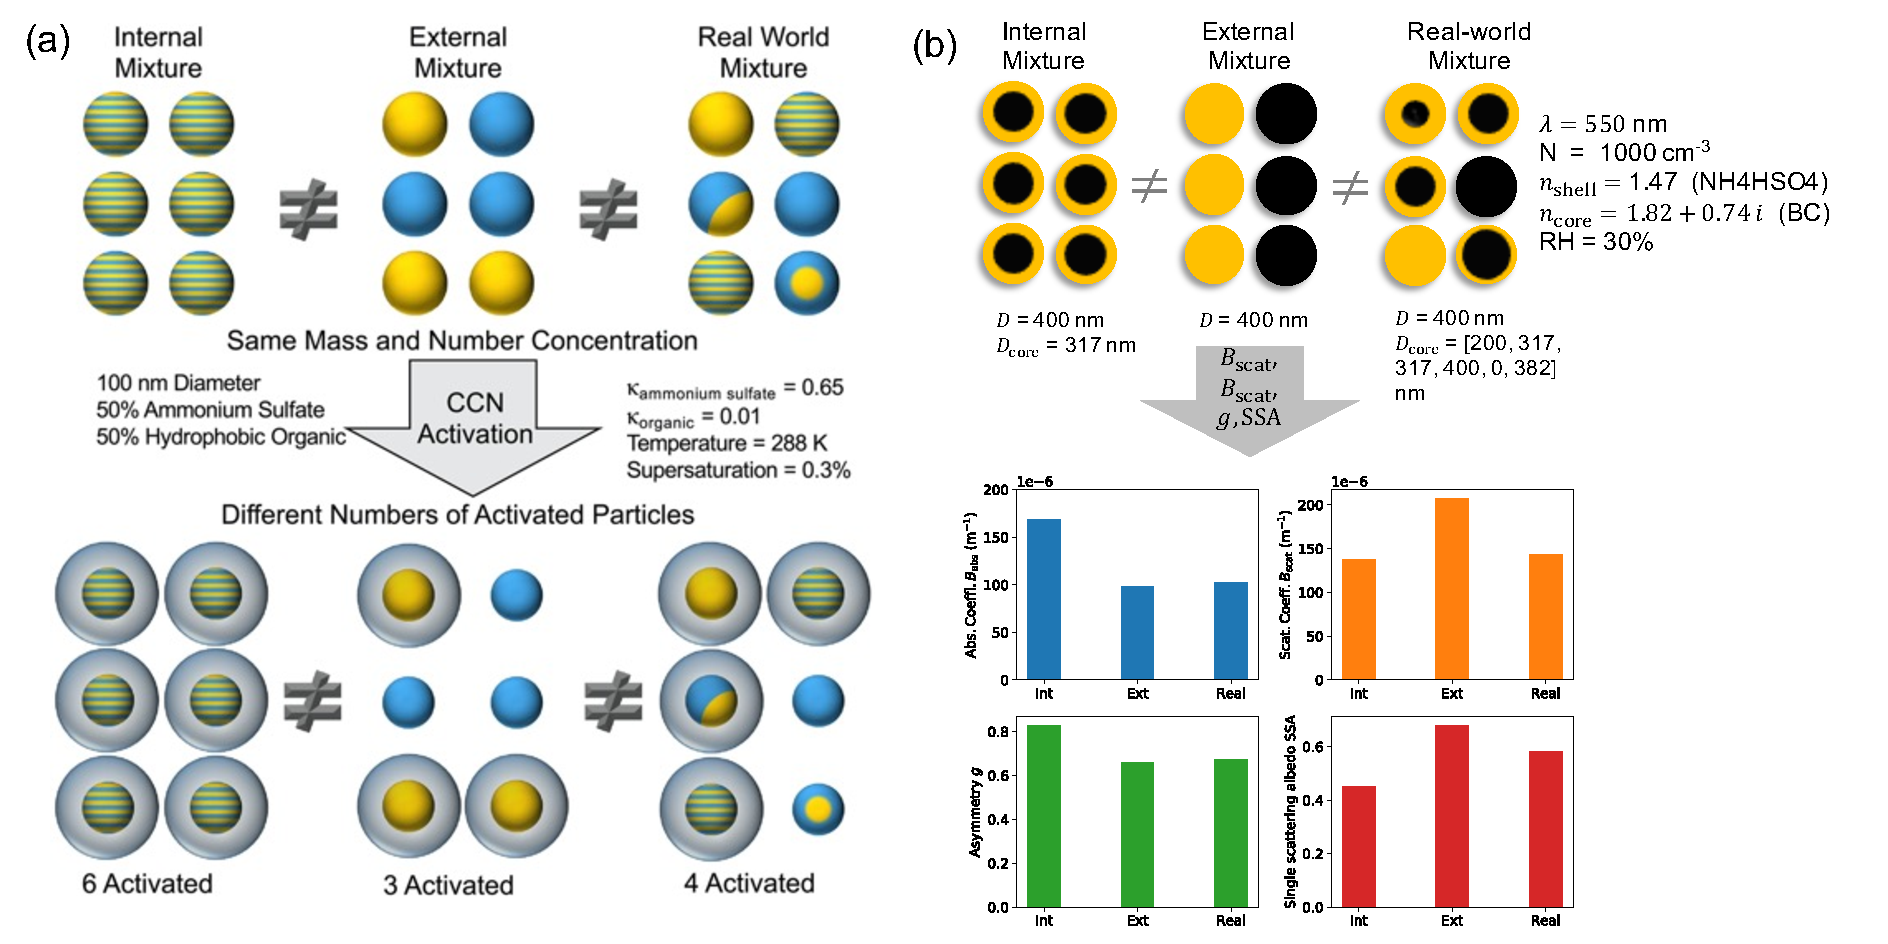
\includegraphics[scale=0.60]{chap1_figs/thesis_chap1_fig3.pdf}
	\caption{Aerosol mixing state effects on (a) activation
          ability and (b) optical values. (a) is adapted from
          \cite{Riemer2019}.}
	\label{fig:chap1-chi-climate}
\end{figure}

The effects of mixing state on aerosol activation potential has been
investigated through closure studies. An aerosol/CCN closure study is
conducted by comparing the observed and predicted CCN concentrations
at a given supersaturation level. The prediction is usually made by
applying K\"ohler theory, using the measured dry particle size
distributions and chemical composition information as input, with
assumptions in mixing state to examine its effects.
\citet{broekhuizen2006closure} performed such a closure study for
aerosol samples from downtown Toronto at 0.58\% supersaturation, and
they found the internal mixture assumptions overpredicted CCN
concentrations by 0.12$\pm$0.05 \textcolor{red}{what unit is
  this?}. Using the CCN sampled from 2010 CalNex field campaign,
\citet{moore2012hygroscopicity} also found internal mixture resulted
in 30--75\% overprediction of CCN concentration. \textcolor{red}{There
  is a paper by Barbara Ervens that would be good to cite here as
  well.}

As for the effects on aerosol optical properties, we can apply the
same strategy as in Fig~\ref{fig:chap1-chi-climate}(a) to explain the
relevance of mixing state. Figure~\ref{fig:chap1-chi-climate}(b) shows
the populations with the same amount of absorbing species (BC) and
non-absorbing species ($\rm NH_4HSO_4$), but with different mixing
states. As a result, the optical properties, including single
scattering albedo (SSA), volume scattering coefficients ($\beta_{\rm
  abs}$) and volume absorption coefficients ($\beta_{\rm abs}$) are
different and can lead to different radiative forcing.

The effects of aerosol mixing state on its optical properties can be
more complicated if considering aerosol water uptake and particle
shapes. In a humidified environment, water update of a particle
depends strongly on its composition because of the dependence of
hygroscopicity on the chemical species, which is important for
scattering \citep{MichelFlores2012, Zieger2013, Titos2014,
  Titos2016}. Studies showed, compared with a dry environment, the
scattering ability can be enhanced by a factor of 1.6 at the
environment with RH of 85\% \citep{Burgos2020}. As for particle
shapes, the distribution of the diverse species {\rm within} a
particle is important in determining optical values. For particles
without strong absorber, i.e. BC, a volume-mixing rule can be used to
calculate the overall refractive index of the particle. When the
particle contains BC, assuming a core-shell configuration has been
shown to be more accurate \citep{Bond2006} than assuming a well-mixed
for which a volume-mixing rule can be used. The absorption enhancement
of BC-contained particles due to its coatings have been widely
investigated \citep{Moffet2009,Liu2017, wu2020light}. The distribution
of the non-absorbing species over the population where found to be the
main sources for the discrepancies between the simulated and observed
optical values \citep{Fierce2016, Fierce2020}. That is, in order to
simulate absorption enhancement correctly, it is important to know the
coating thinkness for a given population of BC cores. In particular,
assuming an internal mixture (where larger BC cores receive thicker
coatings) leads to a systematic overestimation of the absorption
enhancement.

\textcolor{red}{Need to add something on more advanced optical models,
  T-matrix and DDA.}

\section{Aerosol mixing state evolution}  
Aerosol mixing evolution in the atmosphere involves several
processes. It is important to recognize that, at the time of emission,
particles can already be a mixture of different species. For example,
particles emitted from diesel engines are mixture of BC, primary
organics and sulfate, and sea-spray aerosols are a mixture of sodium
chloride and organics \citep{cheung2010emissions,
  kirpes2018secondary}. Once emitted, the mixing state can be further
modified by condensation of organic or inorganic low-volatility
compounds.
%Heterogeneous reactions between gas-phase reactants and
%condensed-phase surface can be faster than reactions in gas-phase,
%and one important reaction is the ozone depletion by chlorine radials
%produced from heterogeneous reactions between chlorofluorocarbons and
%polar cloud surface \citep{davies2018heterogeneous}.
Coagulation between particles is an efficient process for changing
particle number concentration, and Brownian coagulation was shown to
be the main reason for the rapid evolution of soot particle size
distribution near a highway \citep{jacobson2004evolution}. The
coagulation process alone will make the particle composition more
similar, and particle population undergoing coagulation will become
more internally mixed \citep{Riemer2013a}.

The processes of condensation and coagulation outlined above are
relevant for a cloud-free environment, however, since the global cloud
coverage is on average more than 60\%
\citep{stubenrauch2013assessment}, the aerosol evolution in clouds is
also an important contributor during the lifetime of aerosol
populations, and motivates the work presented in Chapter~\ref{xx} of
this thesis. Figure~\ref{fig:chap1-aq-proc} shows the chemical and
physical processes particles experience in fogs and clouds. When the
atmosphere reaches supersaturation, particles with critical
supersaturation lower than the environment supersaturation are
activated as cloud droplets and undergo nucleation scavenging. For
these activated particles, the absorbed water facilitates aqueous
chemical reactions. Gas species dissolve in the cloud droplet, and if
both liquid and ice phases exist in the cloud, species partition
between the two phases and the retention coefficients in the liquid
phase are varied. When cloud droplets grow to rain droplets, they
precipitate. During precipitation, small interstitial aerosol
particles can be collected by these large droplets and impaction
scavenging occurs. For clouds with strong convection, gas and particle
species are vertically redistributed by convective transport.

\begin{figure}
	\centering
	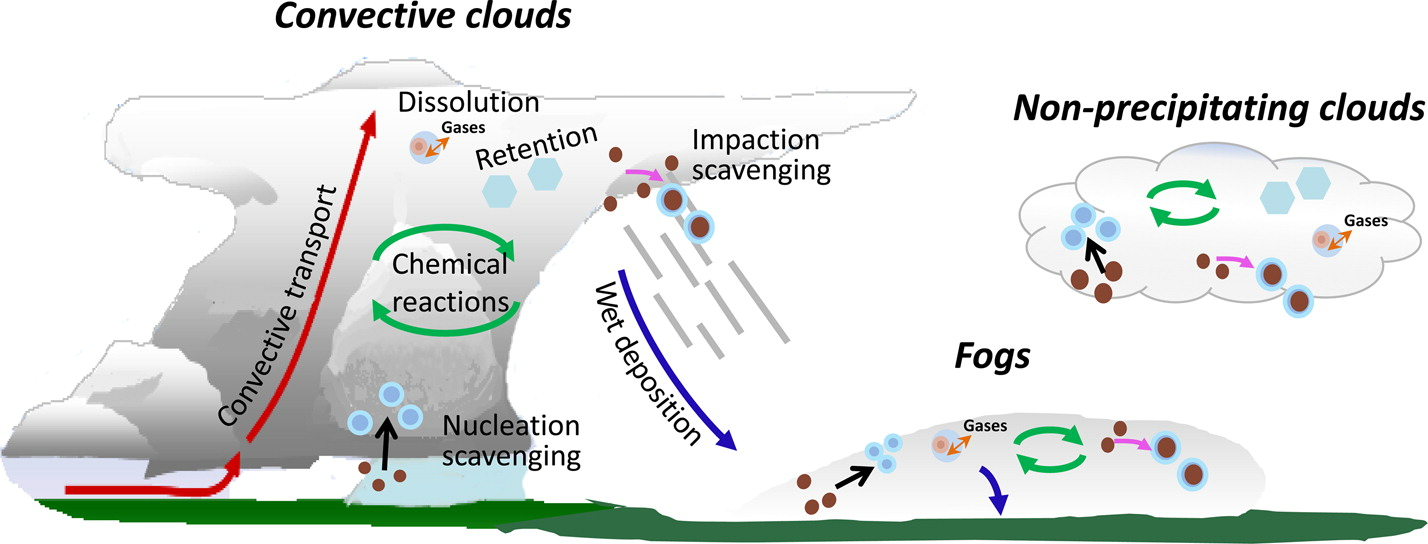
\includegraphics[scale=1.0]{chap1_figs/thesis_chap1_fig4.jpeg}
	\caption{Chemical and physical processes involved in fogs and
          clouds, adapted from \cite{ervens2015modeling}.}
	\label{fig:chap1-aq-proc}
\end{figure}

The aqueous phase in clouds provides an efficient medium for sulfate
formation. Globally, more than 50\% of sulfate forms through in-cloud
oxidation and the formation rates of aqueous reactions, $\rm SO_2$
oxidation by $\rm H_2O_2$ and $\rm O_3$, are more effective than
through OH oxidation in gas phase \citep{kreidenweis2003modification,
  rasch2000description}. Other aqueous sulfate formation mechanisms,
such as the reactions catalyzed by Transition Metal Ions (TMI), can
also be important. For example, reaction cycles involving TMI have
been shown to be the dominant pathway for sulfate formation in the
samples collected during HCCT-2010 field campaign
\citep{harris2012sulfur, harris2013enhanced}.

%Reaction rates of aqueous processes rely on cloud properties and the
%importance of different pathways differs at various cloud types.
%\citet{straub2007chemical}, analyzing the marine stratocumulus cloud
%samples collected over eastern Pacific Ocean during DYCOMS-II field
%campaign, found $\rm SO_2$ oxidized by $\rm H_2O_2$ is the dominant
%reaction for sulfate production.
In addition to sulfate, aqueous reactions can also form SOA. Globally,
SOA produced from aqueous pathway can reach to 20--30 Tg·$\rm
yr^{-1}$. Glyoxal, methylglyoxal, glycolaldehyde and acetic acid can
act as the precursors for aqueous SOA \citep{liu2012global}. As for
the oxidants, besides hydroxyl radical, which is the dominant oxidant
for SOA formation at gas phase, aqueous environment can provide
several other efficient oxidants, such as peroxyl radicals, peroxides
and triplet excited states of organic compounds ($^{3}\textrm{C}^*$)
\citep{mcneill2015aqueous, ervens2011secondary}. Using simulated
sunlight UV, \citet{smith2014secondary} found phenols can be rapidly
oxidized by $^{3}\textrm{C}^*$ to produce low-volatility SOA .

The aerosol size distribution evolves after the formation of aqueous
inorganic and organic species. The characteristic ``Hoppel minimum''
describes the gap between two particle distribution modes at
approximately 0.02--0.03 and 0.08--0.15~$\rm \mu m$
\citet{hoppel1986effect} evident in particle populations processed by
non-precipitating clouds. After being described for the first time by
\citet{hoppel1985effect}, this phenomena has further been observed for
aerosol populations in different regions, such as during the VOCALS
campaign over west Chilean coast and the MASE campaign at the central
California coast \citep{kleinman2012aerosol, hudson2015cloud}. Besides
the formation of secondary aerosol through aqueous phase reactions,
particle size distributions also changes due to coagulation between
interstitial particles and cloud
droplets. \citet{pierce2015importance} found that this process can
reduce total particle number concentration by 10--15\% globally.

The evolution of mixing state in turn affects the aerosols'
climate-related properties. \citet{Ching2016} found that for polluted
environments where BC-containing particles age quickly, increased BC
emissions result in larger cloud droplet number concentrations (even
though fresh BC particles are poor CCN). Aerosol optical properties
are altered as mixing state evolves, especially for BC-contained
particles. As mentioned above, the absorption enhancement of
BC-containing particles due to coatings of non-absorbing species are
widely confirmed by models, laboratory studies and field observations
\citep{Moffet2009,Liu2017,wu2020light,Fierce2020}.

Considering the importance of mixing state for describing an aerosol
population, a qualitative description using the terms, such as
internal or external mixture, are limited in quantifying the effects
of mixing state. \citet{Riemer2013a}, based on the theory of
information-theoretic entropy, developed the index $\chi$ to quantify
aerosol population mixing state. The index $\chi$ is the ratio between
average particle diversity $D_{\alpha}$ and bulk diversity
$D_{\gamma}$. By using particle mass measurement data, these metrics
were successfully proved to be capable of explaining the aerosol aging
processes \citep{Healy2014}. They are also an important framework for
our analyses presented in Chapter~\ref{xx} and Chapter~\ref{xx}.


\section{Aerosol modeling approaches}
The application of a variety of aerosol measurement techniques helps
advance our understanding of aerosol particles, and we know that the
observed particles are the consequence of multiple chemical and
physical processes. By using numerical models, we can isolate the
underlying individual processes, and predict what will happen if
certain processes change. Considering the wide range of chemical
species and particle sizes in an aerosol population, it is hard for a
single model to represent all possible processes the population can
experience during its lifetime, from emission to deposition, and
balance need to be reached between model accuracy and computational
efficiency. This section summarizes the current aerosol modeling
approaches from simplistic bulk methods used in some global models to
comprehensive particle-resolved models used in box model. We will
focus on how these models deal with aerosol mixing state and its
implication for aerosol-related climate properties.

\subsection{Bulk models}
The simplest aerosol modeling approach is the so-called bulk
method. Aerosol populations are represented by the mass concentrations
of several common aerosol species, such as sulfate, BC, organic
aerosol, dust and sea salt, and these species are treated as external
mixtures in the bulk without detailed information about how the
species may be mixed with each other. Rather than tracking the aerosol
evolution through microphysical processes, this approach prescribes
the aerosol size distribution from climatologal data. This approach is
computationally very efficient and applied by several global models,
such as GOCART \citep{chin2000atmospheric} and TM5
\citep{vignati2010sources}.

\textcolor{red}{Add the figure for the bulk model to figure 1.5. I've
  put it in the figures directory.}

\subsection{Modal models}
A more advanced approach is representing the aerosol populations by
several overlapping distributions, also called modes,as shown in
Fig.~\ref{fig:chap1-aerosol-model}(a). A modal model tracks the size
distribution evolution of the modes. Each mode can contain a variety
of aerosol species. Within each mode, all species are assumed to be
internally mixed. Since the modes can overlap in certain size ranges,
mixing state can be represented at least in a simplified way,
especially when many modes are used \citep{Bauer2008}
\textcolor{red}{Add ref to MATRIX model}. Lognormal functions are
typically used to represent the number distribution of each mode as
follows:
\begin{equation}
\centering
    n({\rm log}D_p) = \sum_{i=1}^{m}\frac{N_i}{\sqrt{2\pi}{\rm log}\sigma_i}{\rm exp}(-\frac{({\rm log}D-{\rm log}{\overline{D}_i})^2}{2{\rm log}^2\sigma_i}),
\end{equation}
where $m$ is the number of modes, $N_i$ is the total number
concentration of mode $i$, $\overline{D}_{i}$ and $\sigma_i$ are the
geometric mean diameter and geometric standard deviation of mode $i$,
respectively.

The number of modes can vary among different models. Aitken,
accumulation and coarse modes are the essential three modes, and this
configuration is for example used in the ECHAM4 global climate model
and in the regional chemistry transport model
\citep{lauer2005simulating,
  binkowski2003models}. \textcolor{red}{better to split up the
  references.} Other models introduce additional modes to better
represent hydrophilic and hydrophobic species. For example, MAM7 used
in the CAM5 global model applies an additional primary carbonaceous
mode that represents primary organic matter and BC, which has lower
hygroscopicity than the accumulation mode \citep{liu2012toward} that
also contains sulfate and SOA. For the three parameters used to
describe the lognormal distribution, standard deviation of each mode
is typically prescribed, and total number concentration and geometric
mean diameter change as the aerosol evolves.

\begin{figure}
	\centering
	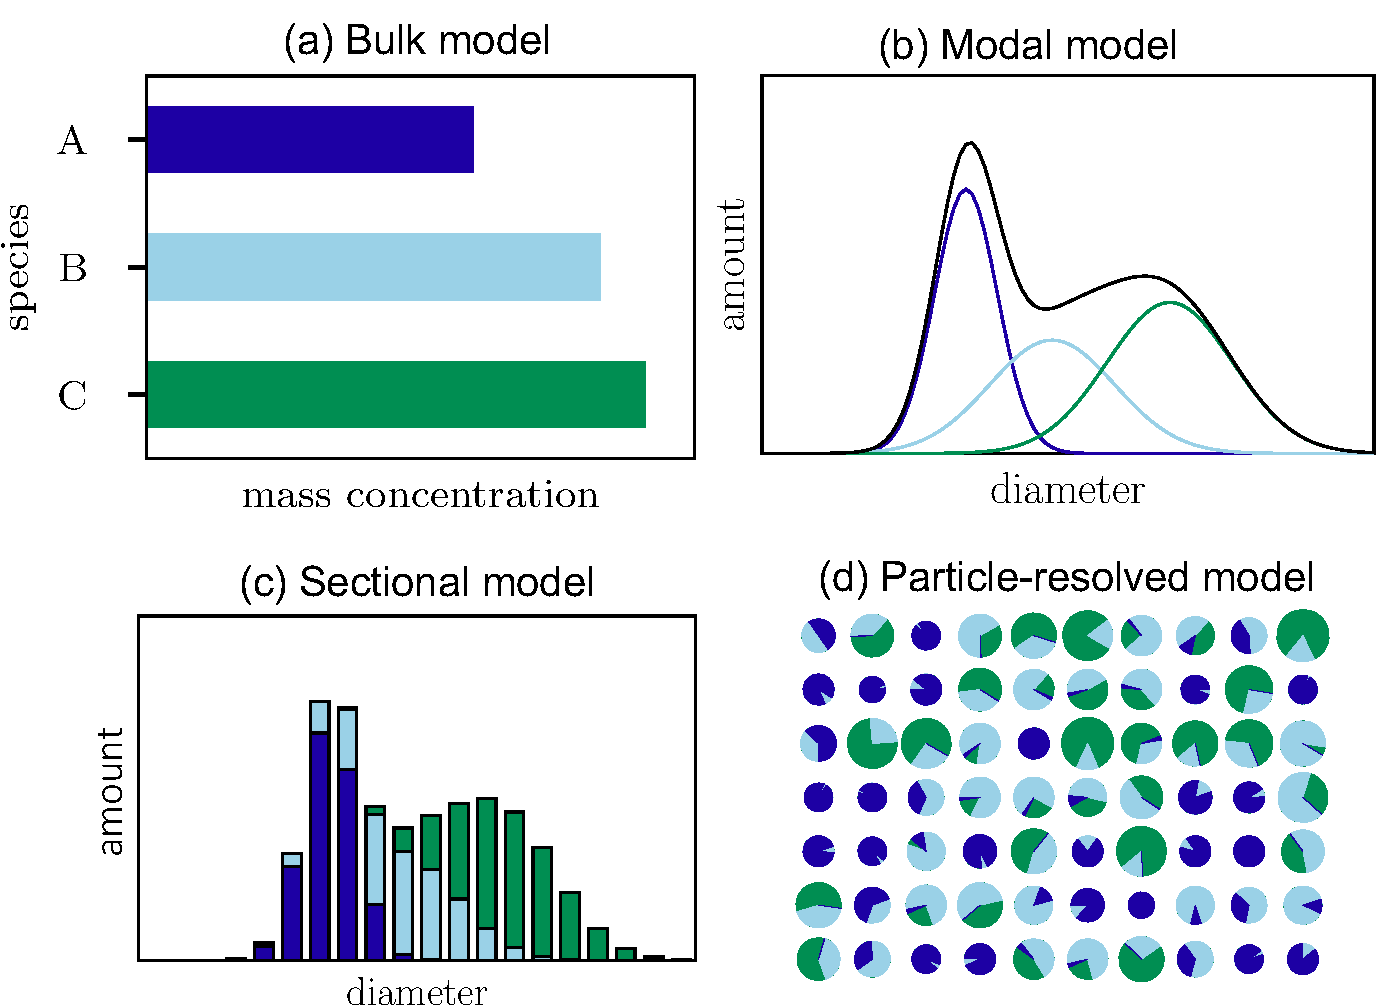
\includegraphics[scale=0.5]{chap1_figs/thesis_chap1_fig5.pdf}
	\caption{Aerosol numerical approaches:(a) Modal model, (b)
          Section model, and (c) Particle-resolved model
          \textcolor{red}{add one more panel for bulk (I added the
            figure already to the repo}}
	\label{fig:chap1-aerosol-model}
\end{figure}

\textcolor{red}{Probably should write out the model acronyms (CAM,
  MOSAIC, ...)}

\subsection{Sectional models}
Similar to modal methods, sectional aerosol models are also
distribution-based. Instead of tracking the population by different
modes, this approach discretizes the distribution into a certain
number of size bins and then track the changes in each bin, as
illustrated in Fig.~\ref{fig:chap1-aerosol-model}(b). Particles are
internally mixed within each bins and the composition can vary between
bins. The sectional approach is widely applied to large-scale
models. For example, the sectional model MOSAIC is extensively used in
WRF-Chem with 4-bin and 8-bin versions available, and proved to
capture the summer particulate matter distribution well over the
Houston region \citep{zaveri2008model,fast2006evolution}. The TOMAS
sectional model is applied to several global chemistry models, such as
GEOS-Chem, and improved its ability in simulating aerosol optical
properties recently through more detail mixing state representation of
BC-contained particles
\citep{adams2002predicting,pierce2013weak,kodros2018size}. TOMAS uses
30 bins and covers the diameter range between 0.01 and 10 $\rm \mu m$.

Most sectional models apply univariate distributions and use
assumptions for the aerosol mixing state in each bin. Some more
advanced schemes have been developed to incorporate more information
within each size bin, especially for representing a variable BC mass
fraction within each size bin. Based on the Model of Aerosol Dynamics,
Reaction, Ionization, and Dissolution (MADRID) module,
\citet{oshima2009aging} developed a two-dimensional sectional scheme
MADRID-BC by adding another dimension for BC mass fraction and
tracking the fraction changes due to condensation/evaporation
processes. Through developing MOSAIC-MIX, \citet{ching2016three}
further extended the sectional model representation by incorporating
another dimension for hygroscopicity, and coagulation process had been
added to evaluate its effects on BC mixing state.

\subsection{Particle-resolved models}
Even though modal and sectional models provide better representation
of particle size distributions than bulk models, aerosol mixing state
still needs to be represented in a simplified way by using internal or
external assumptions. A more advanced representation of aerosol mixing
state is the particle-resolved method, as illustrated in
Fig.~\ref{fig:chap1-aerosol-model}(c). Rather than using distributions
to represent the population, a particle-resolved model samples the
population with discrete computational particles. Specifically, each
particle is represented by an $A$-dimensional vector, where $A$ is the
total species number. The first particle-resolved aerosol model for
the ambient atmosphere was developed by \citet{Riemer2009} and it was
coupled with the MOSAIC module to include gas-particle partitioning
and gas chemistry processes. The model was applied to investigate the
aging process of BC-contained particles in a urban plume environment
and the evolution of ship plume particles \citep{tian2014modeling,
  Ching2016}. Recently, PartMC-MOSAIC had been further coupled with
WRF-chem to track the particle evolution for a large-scale domain
\citep{curtis2017single}. However, MOSAIC only considered aerosol
aging process for subsaturated environments (RH < 100\%). It can not
be used to investigate the chemical processes in a cloud
environment. Extending and applying the PartMC modeling framework to
include aqueous phase chemistry is one of the goal for this
thesis. More details about PartMC will be presented in
Chapter~\ref{xx}.

In summary, the bulk model approach is the most simplified method with
mixing state being represented by an external mixture of different
particle types. Modal and sectional models represent aerosol
populations by distributions. Their ability to describe aerosol mixing
state is limited by the number of modes or bins included in the models
and they still rely on assumptions for mixing state within modes or
bins. With the particle-resolved approach, each computational particle
is explicitly tracked and the mixing state of aerosol population is
accurately represented.

\section{Models for aqueous chemistry simulation }
One of the topics for the thesis is to investigate the impact if
aqueous phase chemistry on aerosol mixing state. The previous section
discussed different approaches to simulate aerosol composition and
represent mixing state. This section summarizes how aqueous phase
chemistry mechanisms are incorporated into models. From particle
activation at nanometer scale to stratocumulus structures over
thousand kilometers, cloud processes cover around $10^{14}$ orders of
magnitude, and it is infeasible for a single model to incorporate all
the related processes. Models with aqueous processes can be divided
into two groups: process model with explicit aerosol microphysics and
complex aqueous chemical mechanisms, and
large-scale model with simplified representation of cloud properties
and processes.

For process models, often used as box/parcel models, aerosol
microphysics is usually well-resolved. Droplet activation is
explicitly described by using K$\rm \ddot{o}$hler
theory. Specifically, particles with critical supersaturation lower
than maximum supersaturation reached in the environment are activated
as droplets \citep{rothenberg2016metamodeling,
  ching2012impacts}. Detailed aqueous chemistry processes can be
incorporated into these cloud parcel models. An example is the cloud
parcel model SPACCIM coupled with the detailed aqueous scheme CAPRAM
(492 species and 1087 reactions in version 3.0). It has been
successfully compared to measurements during the FEBUKO campaign
\citep{wolke2005spaccim}. Since particle size distributions are
commonly described in process models, the modification of the size
distribution after cloud processes can also be captured. The
limitation of these models is the lack of the interactions with the
cloud dynamics. 

It is hard to include such detailed process information in global
models where computational efficiency is very important. Rather than
resolving cloud microphysics explixcitly, cloud properties are
described in a highly parameterized way, by using cloud fraction, with
other diagnosed meterological parameters, for each grid box. Cloud
droplet sizes distributions are usually assumed. For example,
ECHAM5-HAM assumed two bins for the cloud droplets: one bin for
particles with lower ion concentration and the other bin for high ion
concentration. As for the effects of cloud droplets representation on
cloud chemistry, \citet{barth2006importance}, by comparing sectional
and single-size droplet parcel model, found simplified cloud droplet
size representation will lead to biases in simulated formic acid and
formaldehyde concentration. Simplified aqueous mechanisms are also
used and the acidity, which is an important factor for aqueous
chemistry, are fixed at constant value. For example, GEOS-Chem used a
pH of 4.5 for $\rm SO_2$ oxidation reaction by $\rm
O_3$\citep{park2004natural}. Furthermore, assumptions need to be made
to considering the distribution of species produced from aqueous
reactions. For example, in CMAQ, all the non-volatile aqueous-formed
species are added to accumulation mode after cloud dissipates
\citep{binkowski2003models, fahey2017framework}.
 
%\begin{table}
%\setlength\extrarowheight{5pt}
%\centering
%\caption{Overview of acidity, mixing state and optical calculation treatment in different models}
%\label{tab:input}
%\begin{tabular}{ c c c c c}
%	\hline
%	Model acronym  & Model scale &  pH  &  mixing state & Optical calculation  \\
%	\hline
%    CMAQ & Regional & Equilibrium pH & Internal mixture in each mode & \\
%    WRF-Chem (MOSAIC) & Regional  & Equilibrium pH & Internal mixture in each bin &\\
%    GEOS-Chem (TOMAS) & Global & fixed pH at 4.5 & Internal mixture in each bin & \\
%    MOZART & Global & pH based on charge balance &  & \\
%    ECHAM5-HAM & Global & 
%    \begin{tabular}{@{}c@{}}pH based on initial aerosol \\ at small and large droplets\end{tabular} & Internal mixture in each mode & \\
%    PartMC-MOSAIC & 0-D & \begin{tabular}{@{}c@{}}pH based on detailed \\ mechanism at CAPRAM 2.4\end{tabular} & particle-resolved & \\
%	\hline
%   \end{tabular}
% \end{table}
\section{Research questions and thesis organization}
Aerosol particles affect climate forcing through directly altering
radiation and indirectly interactions with clouds. These effects are
dependent on the particles' chemical composition, in other words, the
chemical species mixing state of the aerosol population. The objective
of this dissertation includes two parts: quantifying cloud chemical
processes and their impact on mixing state, and quantifying the
effects of aerosol mixing state on aerosol optical properties. 

For the first part, I will focus on the following scientific
questions: (1.1) Is particle-resolved approach capable of simulating
the complicated aqueous processes? (1.2) To what extent does cloud
processing change the aerosol mixing state of the population that
entered the cloud?  (1.3) How does this change the cloud condensation
number concentration and optical properties? (1.4) What is the
implication of coagulation between the interstitial particles and
cloud droplets for mixing state of aerosol population?

\textcolor{red}{1.1 is difficult to evaluate -- people might think we
  should compare more to measurements. I would only have the other
  three.}

For the second part, the following two questions will be addressed:
(2.1) What are the errors in aerosol optical properties introduced by
internal mixture assumptions used in sectional models? (2.2) How does
this error depend on relative humidity and associated water uptake of
the aerosol?

Both objectives are addressed with a particle-resolved modeling
approach. Chapter 2 describes the coupling of the particle-resolved
model PartMC-MOSAIC with the aqueous mechanism
CAPRAM. Chapter~\ref{xx} also presents the results from idealized
model simulations to confirm expected sensitivities of sulfate
formation to model input parameters. The findings will be concluded in
the preparing paper ``Sensitivity of sulfate in-cloud chemistry to
aerosol acidity variability and mixing state'' for \textit{Aerosol
  Science and Technology}.

\textcolor{red}{not sure about mentioning this paper here. There is a
  lot of work still to be done to bring this to publication. It's not
  impossible, just not immediately imminent.}

\textcolor{red}{don't hardcode references to chapters.}

Chapter 3 investigates the cloud processing effects on aerosol
properties. In this work, I used a typical urban plume particle
population to experience several idealized cloud cycles to determine
the changes of aerosol mixing state and quantify the changes of
aerosol microphysical and optical properties after the cloud
evaporates. Another simulation is conducted to identify the role of
coagulation between cloud droplets and interstitial particles. This
chapter will answer questions 1.2--1.4. A paper entitled ``The impacts
of cloud processing on resuspended aerosol particles after cloud
evaporation'', which is in review for \textit{Journal of Geophysical
  Research-Atmosphere}, summarizes the results on the changes of
aerosol microphysical properties after cloud processing. Another
paper, which is entitled with ``Quantifying the Effects of Cloud
Processing on Aerosol Optical Properties Using a Particle-Resolved
Model'' about the changes of optical properties after cloud
processing, is in preparation for \textit{Aerosol Science and
  Technology}.

Chapter 4 evaluates the error in aerosol absorption and scattering,
introduced by the internal mixture assumptions used in sectional
aerosol models. The error is quantified by comparing the aerosol
optical value differences between reference populations created by
running particle-resolved model and sensitivity populations with
reduced representation of mixing state created by
composition-averaging methods. This chapter will answer the two
questions in second part and the work is in preparation for
\textit{Atmospheric Chemistry and Physics}, entitled ``Quantifying the
effects of mixing state on aerosol optical properties''.

Chapter 5 summaries the main findings of these works and implications
for resolving aerosol mixing state in the future for global models.
%%%%%%%%%%%%%%%%%%%%%%%%%%%%%
%%%%%%%%%Chapter 2%%%%%%%%%%%
%%%%%%%%%%%%%%%%%%%%%%%%%%%%%
\chapter{Particle-resolved modeling of aqueous-phase chemistry}

This chapter presented the application of PartMC as a particle-resolved aqueous-phase chemistry model. In this work, I first described PartMC-MOSAIC model, and the coupled cloud parcel and aqueous chemistry module. Then, I evaluated the coupled model by comparing with other size-resolved and bulk cloud chemistry models. Furthermore, I designed ensemble scenarios to investigate the efficiency of different aqueous sulfate formation pathways. Another group of ensemble scenarios are conducted by adding transition metal ions (TMI) in the population to determine the efficiency of sulfur oxidation reactions catalyzed by TMI. 

\label{chap2:mon}
%%% Suggested section heads:
\section{Introduction}

Clouds cover around 70$\%$ of the earth \citep{Stubenrauch2013}. The coexistence of species multi-phases in the cloud provides a favorite medium for the interactions between different phases \citep{Deguillaume2005}. Gas can transfer to the liquid droplets through thermodynamic processes and undergoes heterogeneous chemistry, which in return affect the particle activation potentials \citep{Farmer2015, Henning2014}. Oxidation of dissolved gases in the aqueous phase can contribute to a large fraction of particle species, especially for the secondary inorganic and organic species. Globally, over 50\% of sulfate are produced through aqueous reactions \citep{Philip2014, Roth2016}. The goal of this work is to investigate the roles of different aqueous sulfate formation pathways. 

Particles with different composition and size experience different net effects from aqueous chemical processing. First, per-particle properties affect cloud processes by determining which particle can be activated as cloud droplets. The activation potential of particles is determined by its size and compositions, and CCN closure studies indicated the simplified assumptions of particle mixture in the population can lead to simulated CCN concentration bias \citep{Broekhuizen2006, Bhattu2015}. Second, particle diversity affects aqueous reaction rates. Aqueous sulfate formation reactions are highly pH-dependent, and the reaction rates for particles with different acidity can vary in several orders. For example, transition metal ions (TMI), including Fe and Mn ions, which are mostly originated from mineral dust \citep{alexander2009transition}, can catalyze aqueous sulfate oxidation reactions. The related pathways can become dominant when pH is larger than 6.0 \citep{Seinfeld2006a}. It had been proved that at some cloud events, $\rm SO_2$ oxidation reactions catalyzed by coarse mineral dust TMI can be more efficient than $\rm H_2O_2$ pathway \citep{Harris2013a, Harris2014}. 

Despite the importance of particle heterogeneity in aqueous chemistry, most regional or global models used simplified assumptions to simulate aqueous processes. For global chemistry model GEOS-Chem, less than 10 dissolved species are used to calculate acidity \citep{alexander2012isotopic}.
For regional model CMAQ, cloud chemistry processes are tracked by three lognormal modes, neglecting the heterogeneity inside each mode \citep{fahey2017framework}. In this work, I applied the particle-resolved model PartMC-MOSAIC \citep{Riemer2009, Zaveri2010a}, which can track particles individually. This approach is well-suited for this problem because it can track the evolution of compositions and sizes of individual aerosol particles without averaging their composition within size bins or modes. The model had been widely used to study particle aging processes in cloud-free environment \citep{ching2012impacts, Ching2016}, and in current work, I first applied the model with cloud chemistry processes. 

This work was structured as follows: Section~\ref{chap2.2} described the models used in current work and Sect.~\ref{chap2.3} evaluated the particle-resolved aqueous chemistry model by comparing with other widely-used models. Section~\ref{chap2.4} investigated the role of different aqueous sulfate formation pathways by analyzing the ensemble cases and the role of TMI pathway is further explored in Sect.~\ref{chap2.5}. Findings were concluded in Sect.~\ref{chap2.6}. 

\section{Model description and simulations setup}
\label{chap2.2}
Following the two-step strategy described in \citet{ching2012impacts}, I designed the cloud chemistry experiment by exposing aerosol populations in a cloud environment, as figure~\ref{chap2-fig1-frame} illustrates. For the first step, Isimulated urban plume scenarios that produced populations with a wide variety of aerosol mixing states using a particle-resolved model PartMC-MOSAIC in a cloud-free environment. These simulated aerosol populations were then used as the input for cloud parcel simulations, including aqueous chemistry, in step 2. Details of PartMC-MOSAIC, cloud parcel model and aqueous chemistry are described in the following sections.

\begin{figure}[ht]
    \centering 
    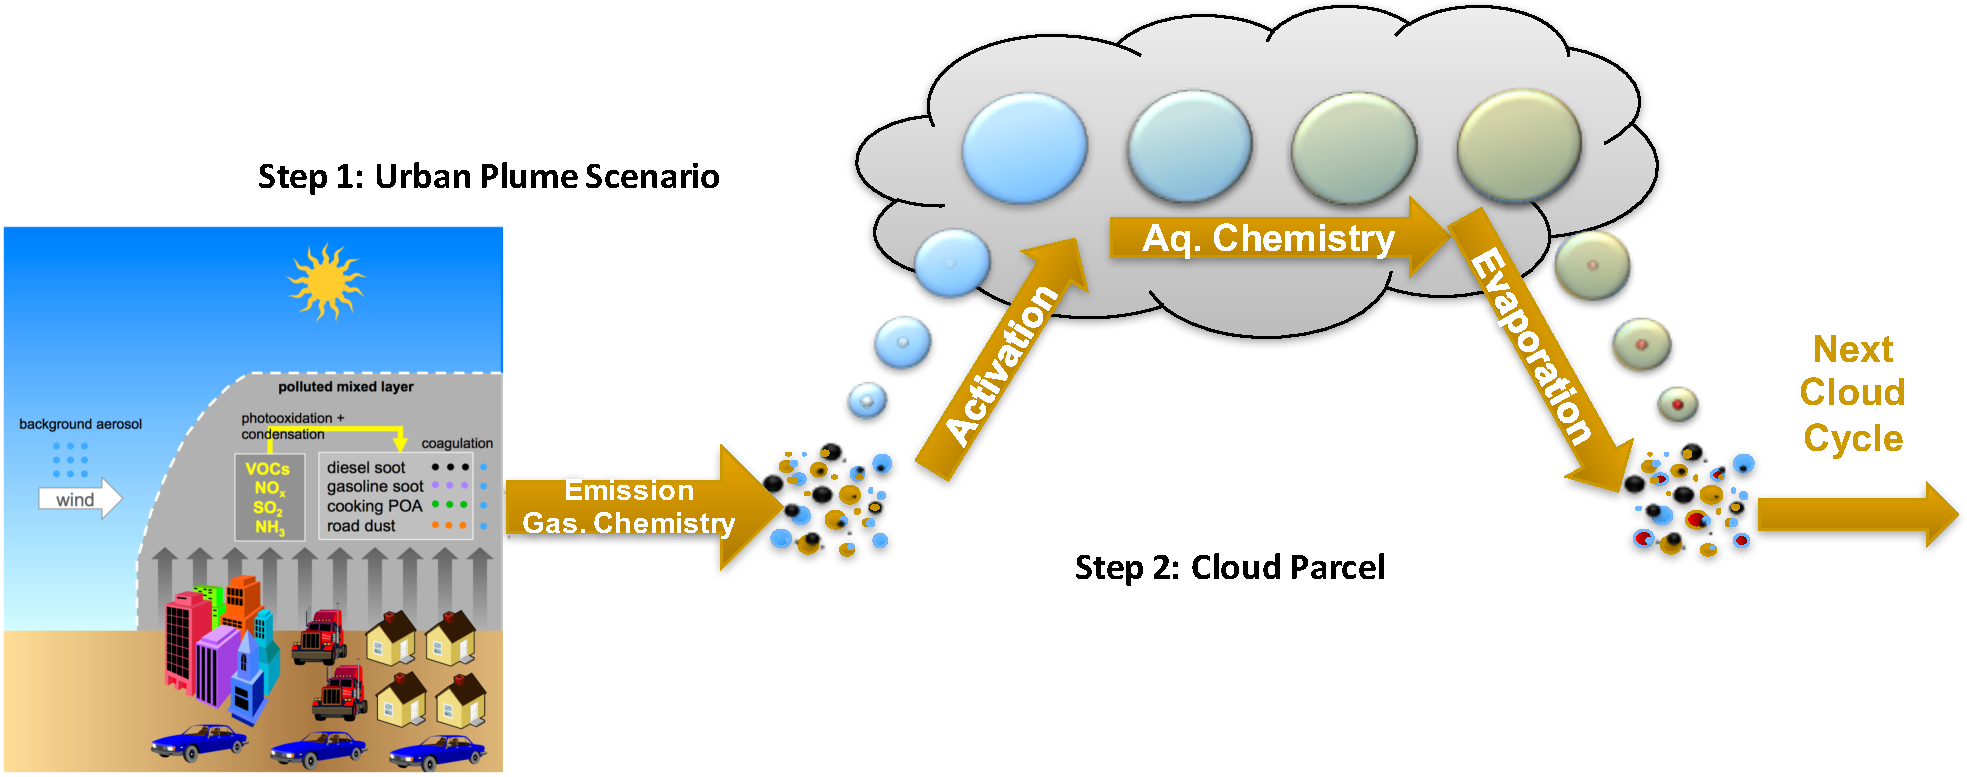
\includegraphics[scale=0.4]{chap2_figs/chap2-fig1-frame.pdf}
    \caption{Two-step cloud chemistry experiment framework}
    \label{chap2-fig1-frame}
\end{figure}

\subsection{Particle-resolved model PartMC-MOSAIC}
PartMC-MOSAIC (Particle Monte Carlo-Model for Simulating Aerosol Interactions and Chemistry) is a Lagrangian box model which simulates the evolution of individual particles by different processes. The evolution is simulated in a well-mixed computational volume and the particle spatial positions are not stored. Compositions of each particle are explicitly tracked by representing the particle as an $A$-dimension vector $\vec{\mu}^i \in \mathbb{R}^A$ with components ($\vec{\mu}_1^i,\vec{\mu}_2^i,...,\vec{\mu}_A^i$), where $\vec{\mu}_a^i$ is the mass of species $a$ in particle $i$, with $a$ = $1,...,A$ and $i$ = $1,...,N$. The evolution for aerosol number concentration with species mass $\mu$ at time $t$, $n(\vec{\mu},t)$, is described by: 
\begin{equation}
\begin{aligned}
 \frac{\partial n(\vec{\mu},t)}{\partial t} &= \underbrace{\frac{1}{2}\int_0^{\mu_1}\int_0^{\mu_2}...\int_0^{\mu_A} K(\vec{\mu}',\vec{\mu}-\vec{\mu}')n(\vec{\mu}',t)n(\vec{u}-\vec{u}',t)d{\mu_1}'d{\mu_2}'...d{\mu_A}'}_\text{coagulation gain}\\
& - \underbrace{\int_0^\infty\int_0^\infty...\int_0^\infty K(\vec{\mu},\vec{\mu}')n(\vec{\mu},t)n(\vec{\mu}',t)d\mu_1'd\mu_2'...d\mu_A' }_\text{coagulation loss} + \underbrace{\dot{n}_{\rm emit}(\vec{\mu},t)}_\text{emission} + \underbrace{\lambda_{\rm dil}(t)(n_{\rm back}(\vec{u},t))-n(\vec{\mu},t)}_\text{dilution}\\
&-\underbrace{\sum_{i=1}^{C}\frac{\partial}{\partial\mu_i}(c_iI_i(\vec{\mu},\vec{g},t))n(\vec{\mu,t})}_\text{gas-particle transfer} - \underbrace{\frac{\partial}{\partial\mu_{C+1}}(c_wI_w)(\vec{\mu},\vec{g},t))n(\vec{\mu,t})}_\text{water transfer} + \underbrace{\frac{1}{\rho_{\rm dry}(t)}\frac{d\rho_{\rm dry}(t)}{dt}n(\vec{\mu},t)}_\text{air density change},
\end{aligned}
\label{eq:partmc}
\end{equation}
where $K$ is the coagulation rate between the particles, $\dot{n}_{\rm emit}(\vec{\mu},t)$ is the emitting distribution of species $\vec{\mu}$, $\lambda_{\rm dil}$ is the dilution rate with background species concentration $n_{\rm back}$, $c_i$ is the gas to particle conversion rate, $I_i$ is the gas species condensation flux, $c_{\rm w}$ is the gas to water conversion rate and $I_{\rm w}$ is the water condensation flux. More details of the equation can refer to \citet{Riemer2009}.

The evolution processes involved in the equation~\ref{eq:partmc} alter the aerosol population in two mechanisms. By adding or removing particles from the population, emission, dilution and coagulation processes modify the number concentration of the population and these processes are accomplished by PartMC with a stochastic Monte Carlo approach. While on the other hand, composition of each particle can be altered by species condensation and evaporation, which are explicitly simulated by state-of-art aerosol chemistry module MOSAIC. In MOSAIC, gas phase reactions are accomplished by carbon bond mechanism CBM-Z, 77~species and 142~reactions are included \citep{Zaveri1999}. Key aerosol species are treated, including $\rm SO_4^{2-}$, $\rm NO_3^-$, $\rm NH_4^+$, BC, primary organic aerosol (POA) and secondary organic aerosol (SOA). SOA treatment is based on SORGAM scheme \citep{schell2001modeling}. In current version, model includes four SOA species (ARO1, ARO2, ALK1, OLE1) oxidized from anthropogenic volatile organic compounds (VOCs) and four other SOA species (LIM1, LIM2, API1, API2) oxidized from biogenic VOCs \citep{ching2012impacts}. Activity coefficients of electrolytes and ions in aqueous solutions are estimated by multicomponent Taylor expansion method (MTEM), and intraparticle solid-liquid partitioning are treated by Multicomponent Equilibrium Solver for Aerosols (MESA) \citep{zaveri2005computationally}. However, MOSAIC only considered the reactions occurred in an unsaturated environment (RH < 100\%) and therefore we were not able to address the change within the cloud. This is the contribution of this work. 

PartMC-MOSAIC had been applied to analyze the particle evolution at different environment. For example, \citet{Zaveri2010a} found particle optical absorption increased by 40\% during a 48-hour idealized urban plume condition due to the aging of BC-contained particles. \citet{tian2014modeling} used the model to investigate the processes responsible for the particle number concentration change in a ship plume environment and evaluated the effects of different aging process on particle CCN properties. PartMC-MOSAIC was also used as a benchmark model to quantify the errors in aerosol optical and microphysical properties introduced by simplified mixing state assumptions commonly used in other aerosol models \citep{Zaveri2010a, ching2012impacts, Fierce2017}. PartMC-MOSAIC was further coupled with a cloud parcel model to investigate the effects of mixing state on cloud droplet properties \citep{ching2012impacts, Ching2016}, and the cloud parcel model will be discussed in detail in section~\ref{section:cloud-parcel-model} because this model was applied for the research both in  this chapter and chapter~3. 

\subsection{Cloud parcel model}
\label{section:cloud-parcel-model}
The cloud parcel model coupled with PartMC-MOSAIC is an zero-dimensional adiabatic model. It simulates the particle activation and condensation growth in a rising air parcel and tracks the changes of environment saturation due to the growth of particles and temperature change. Specifically, for a population with $N$ particles of diameter $D_i$, both the growth rate of $D_i$ and the change of environment saturation $S_v$ are diagnosed, which sums to $N$ + 1 state variables to be numerically solved by the model. To focus on the effects of chemical compositions on cloud droplets formation, entrainment, surface tension effects on droplets growth are not included in the model. This section briefly introduces the main equations solved by the parcel model. See \citet{ching2012impacts} for more detailed description of the model. 

During the condensational growth process, the chemical compositions of particle are assumed to be constant and only the water content of the particle alters. The growth rate of particle $i$ is calculated as
\begin{equation}
\centering
\frac{dD_i}{dt} = \frac{G}{D_i}(S_{\rm v}-S_{\rm eq})
\label{eq:cloud-parcel} 
\end{equation}
where the growth coefficient $G$ and droplet equilibrium supersaturation $S_{\rm eq}$ are
\begin{equation}
\centering
\begin{aligned}
 G & = \frac{4D'_{v,i}M_{\rm w}P^0}{\rho_{\rm w}RT}  ,\\
 S_{\rm eq} & = \frac{a_{{\rm w},i}}{1+\delta_i}{\rm exp}(\frac{4M_{\rm w}\sigma_{\rm w}}{\rho_{\rm w}RTD_i}\frac{1}{1+\delta_i} + \frac{\Delta H_{\rm v}M_{\rm w}}{RT}\frac{\delta_i}{1+\delta_i}),
\end{aligned}
\end{equation}
and $D'_{v,i}$ is the modified particle diffusivity, $M_{\rm w}$ and $\rho_{\rm w }$ are the water molecular weight and density, $P^0$ is the saturation vapor pressure, $R$ is the gas constant, $T$ is the environment temperature, $a_{w,i}$ is the water activity of the particle, $\sigma_{\rm w}$ is the water surface tension, $\Delta H_{\rm v}$ is latent heat of vaporization, and $\delta_i$ is defined as 
\begin{equation}
    \delta_i = \frac{\Delta H_{\rm }\rho_{\rm w}}{4k'_{{\rm a},i}T}D_i\frac{dD_i}{dt},
\end{equation}
where $k'_{{\rm a},i}$ is the corrected air thermal conductivity. 

The water activity is calculated by using the parameter $\kappa$ derived by \citet{Petters2007} and can be expressed as
\begin{equation}
\centering
a_{{\rm w},i} = \frac{v_i^{\rm w}}{v_i^{\rm w} + \kappa_i v_i^{\rm dry}},
\label{eq:activity coeff}    
\end{equation}
where $v_i^{\rm w}$ and $v_i^{\rm dry}$ are the volume of water and all the other dry components in particle $i$, respectively. $\kappa_i$ is volume-weighted $\kappa$ of the non-water species. In current model, we used $\kappa$ of 0.65 for ammonium-sulfate-nitrate system, SOA with $\kappa$ = 0.1 and POA with $\kappa$ = 0.001. BC is assumed to be hyrophobic and has $\kappa$ of 0. 

Rather than describing the rising parcel using a constant updraft velocity \citep{Seinfeld2016,rothenberg2016metamodeling}, this parcel model prescribed a constant temperature lapse rate, following the strategy used in \citet{majeed2001microphysics}, to avoid dealing with radiative heating effects and latent heat budget. Pressure is also assumed to be constant. In light of these considerations, the change of environment saturation can be given by
\begin{equation}
    \centering
    \frac{dS_{\rm v}}{dt} = -\sum_{i=1}^{N}\frac{\pi \rho_{\rm w} RT}{2M_{\rm w}P^0V_{\rm comp}}D_i^2\frac{dD_i}{dt} - \frac{1}{P^0}\frac{\partial P^0}{\partial T}S_{\rm v}\frac{dT}{dt}
\end{equation}
where the first term describes the effects due to the radius change of all $N$ particles and the second term is about the temperature change. $V_{\rm comp}$ is the computational volume. 

This coupled model had been applied to investigate the importance of aerosol mixing state for predicting cloud droplets number concentration (CDNC). \citet{ching2012impacts} found, neglecting particle species heterogeneity in size bins resulted in errors in CDNC up to 34\% at the environment with cooling rate of 0.5~\unit{K/min}. By conducting ensemble cloud parcel simulations, \citet{Ching2016} further demonstrated that ignoring BC mixing state can lead to CNDC error of $-$12\% to $+$45\%.

%The coupled model had been used to evaluate the relative importance of particle size and compositions for cloud droplet concentration. 

\subsection{Aqueous chemistry model}
\label{section:aq-chem-model}
In this work, PartMC-MOSAIC was further coupled with an aqueous chemistry module based reduced Chemical Aqueous Phase Radical Mechanism(CAPRAM) version 2.4. The full mechanism in CAPRAM 2.4 includes 439 reactions and 147 species, and a reduced version is also provided to be more computationally efficient, which includes 183 reactions and 113 species \citep{Ervens2003}. The reduced version also contains a comprehensive aqueous mechanism, and deals with the reactions between OH, $\rm HO_2$, $\rm NO_3$, $\rm SO_4$, $\rm Cl_2$,$\rm Br_2$ and $\rm CO_3$ with inorganic (TMI, $\rm NO_3^-$ , $\rm Cl^-$, $\rm Br^-$) and organic reactants with less than two atoms. The constants for thermodynamic and kinetic reactions are listed in Table~\ref{tab:capram}. When coupling CAPRAM with PartMC-MOSAIC, the original gas phase chemistry mechanism, regional atmospheric chemistry modeling (RACM), used in CAPRAM 2.4 is now replaced with CBM-Z in PartMC-MOSAIC. 

\subsection{Ensemble monodisperse settings}
This work is the first application of particle-resolved cloud chemistry model, and I used relative simple aerosol description, that is the monodisperse distribution, to investigate aqueous sulfate processes. More complex populations with lognormal distribution and the role of other cloud processes, such as coagulation between interstitial particles and cloud droplets, are explored in next chapter. 

The goal of this chapter will focus on the following questions: (1) Is particle-resolved approach capable of capturing the various roles of aqueous sulfate formation pathways under different environment? (2) What is the role of TMI pathway for aqueous sulfate formation? 

To answer the first question, I created a reference scenario ensemble by exposing the monodisperse aerosol populations at different chemical and physical environment, denoted as $P_{\rm ref}$. I set the initial particle size at 100 \unit{nm} composed of ammonium sulfate. Emission and dilution were not included in current simulations. Four important gas species for aqueous sulfate formation, including $\rm O_3$, $\rm H_2O_2$, $\rm NH_3$ and $\rm SO_2$, were perturbed at low, medium and high polluted levels, as listed in table~\ref{TMI-setting}. The $\rm O_3$ and $\rm SO_2$ values of these three levels were based on the national wide urban measurements in China \citep{wang2014spatial}, and $\rm NH_3$ levels were determined from the observations of Houston, U.S. \citep{nowak2010airborne} and Seoul, Korea \citep{phan2013analysis}. The values for $\rm H_2O_2$ were based on the measurements in Guangzhou, China \citep{hua2008atmospheric}. I also set three different temperature rates to provide cloud environment with varied liquid water content, and the corresponded cloud updraft velocity were 1.1, 1.5 and 1.8\unit{m\;s^{-1}} respectively, which represented the conditions of strong convective stratus \citep{peng2005importance}. In total, I simulated $3^5$ = 243 cases in this ensemble scenario.

\begin{table}[ht]
\centering
\caption{Settings for $P_{\rm ref}$ ensemble simulation}
\label{TMI-setting}
\begin{tabular}{c  c c  c}
\hline
Parameters & Low  & Medium & High\\
\hline
$\rm O_3$& 25 & 50 & 75 \\
$\rm H_2O_2$& 0.25 & 0.5 &  1\\
$\rm NH_3$ &2 & 4 & 6 \\
$\rm SO_2$&2&5& 10\\
$\frac{dT}{dt}$ &$-$0.3 &$ -$0.4&$-$0.5\\
\hline
\end{tabular}
\end{table}

The initial RH was 99\% and the simulation lasted 20 minutes. As showed in Fig.~\ref{chap2:ensemrh}, cases with higher temperature lapse rates experienced more rapid increase of liquid water content, while the reached maximum supersaturation were close between the cases. Cloud formed in the first minute and the maximum supersaturation was 0.2\%. 

\begin{figure}[ht]
    \centering 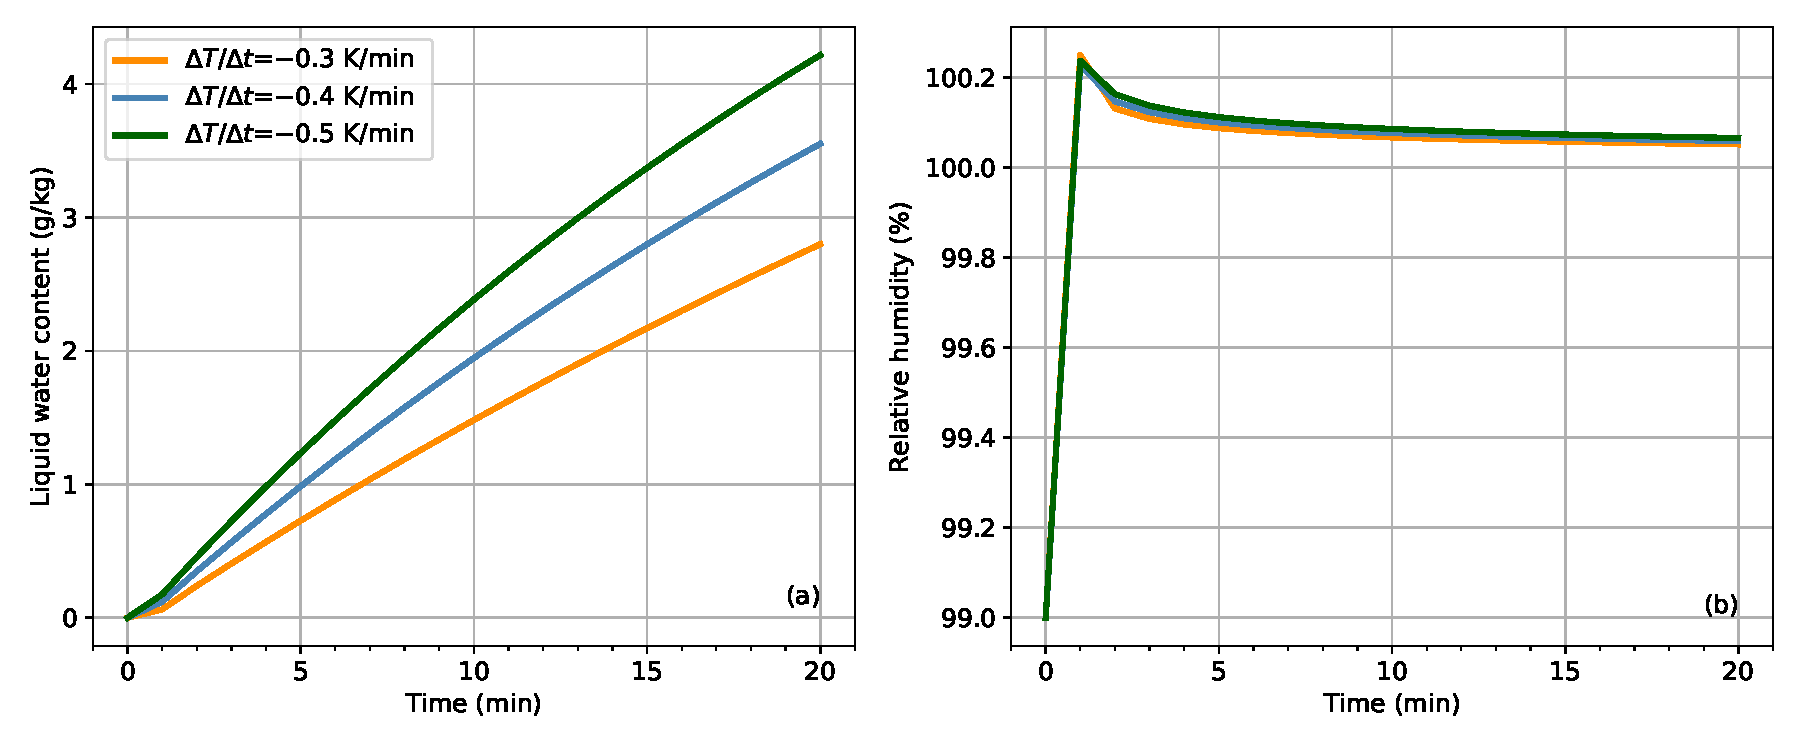
\includegraphics[scale=0.55]{chap2_figs/chap2_mono_lwc_rh.pdf}
    \caption{Time series of (a) liquid waeter content and (b) relative humidity in the ensemble scenarios. Blue, orange and green lines are for the cases with temperature lapse rate of --0.3 \unit{K/min}, --0.4 \unit{K/min} and --0.5 \unit{K/min} respectively.}
    \label{chap2:ensemrh}
\end{figure}

In order to answer the second question, I created another sensitivity scenario ensemble, denoted as $P_{\rm TMI}$ by adding $\rm Fe(II)$ and $\rm Fe(III)$ in the initial aerosol population. I set the mass fraction of $\rm Fe(II)$ and $\rm Fe(III)$ to be 0.05 and 0.01. \citet{deguillaume2004role} found aqueous hydroxide is important for TMI oxidation pathways and the concentration is in the order of $\rm 10^{-13}$~\unit{M}. I achieved this by emitting gas OH at the rate of $2\times 10^{-8}$ \unit{mole/m^2/s}. I also applied the same perturbed parameters as in $P_{\rm sul}$, which results in another 243 cases for $P_{\rm TMI}$. 

\section{Sulfate mechanism verification}
\label{chap2.3}
Before applying the comprehensive particle-resolved aqueous chemistry model to study the role of different aqueous sulfate pathways, I first evaluated it by comparing with the models used in \cite{kreidenweis2003modification}(hereafter, KS2003). In KS2003, several bulk and size-resolved models were used to simulate aqueous sulfate formation in an adiabatic updraft cloud environment. They found significant differences in $\rm SO_2$ oxidation rates between size-resolved and bulk models. This model comparison work provides a benchmark for checking aqueous sulfate mechanisms, and I used the same simulation setting in that work to verify our particle-resolved aqueous chemistry approach. Physical and chemical conditions, including the updraft velocity, temperature change, initial species concentration and chemical equations are all set to the same with values used in KS2003, as listed in table~\ref{setting}. In the models used in KS2003, cloud formed by a constant updraft velocity. But in our model, as mentioned before, we predefined the temperature lapse rate. In order to get the same updraft velocity, we obtained the temperature values of constant updraft velocity at 0.5 from pyrcel model, a zero-dimensional adiabatic cloud parcel model \citep{rothenberg2016metamodeling}. 

\begin{table}[ht]
\centering
\begin{threeparttable}
\caption{Cloud  chemical and physical conditions}
 \begin{tabular}{l c|c l}
 \hline
  Physical parameters & Value (Units) & Chemical parameters ($t = 0$) & Values Units\\
 \hline
 Temperature at $t =0$ & 285.2 (K)&$\rm SO_2$ & 200 (pptv)\\
 Pressure at $t$ = 0 & 950 (mbar)&$\rm NH_3$ & 100 (pptv)\\
 Updraft velocity & 0.5 ($\rm m\,s^{-1}$)&$\rm H_2O_2$ & 500 (pptv)\\
 Cloud water mixing ratio after 2400 s& 2.17 ($\rm g\,kg^{-1}$)&$\rm HNO_3$  & 100 (pptv)\\
 Air density at the cloud base & 1.15 ($\rm kg\,m^{-3}$) & $\rm O_3$ &50 (ppbv)\\
 Cloud base temperature& 284.2 K&$\rm CO_2$ & 360 (ppmv)\\
 Cloud base pressure& 939 (mbar)& $\rm SO_4^{2-}$ & 2 ($\rm \mu g \, m^{-3}$)\\ 
 Relative humidity at $t$ =0 & 95$\rm \%$ & $\rm NH_4^+$ & 0.375 ($\rm \mu g\, m^{-3}$)\\
 \hline
 \label{setting}
\end{tabular}
\end{threeparttable}
\end{table}

Figure~\ref{chap2:ks2003}(a) shows the simulated cloud liquid water content (LWC). PartMC simulated higher LWC changing rate and it may result from the different cloud parcel model settings. As mentioned before, we prescribed a constant temperature lapse rate. But for models used in KS2003, a constant updraft velocity was described. In current simulation, the input temperature profile produced updraft velocity close to 0.5~\unit{m/s}, but still with some fluctuations around 0.1~\unit{m/s}, and this can be the main reason for the LWC differences. Another possible factor is the treatment of droplet surface temperature $T$, which is used to calculate droplet growth rate and it is common for models to assume $T$ equals to environment temperature $T_\infty$. But in our model, we did not use this assumption and the different treatments may also result in the calculated LWC differences.

\begin{figure}[ht]
    \centering 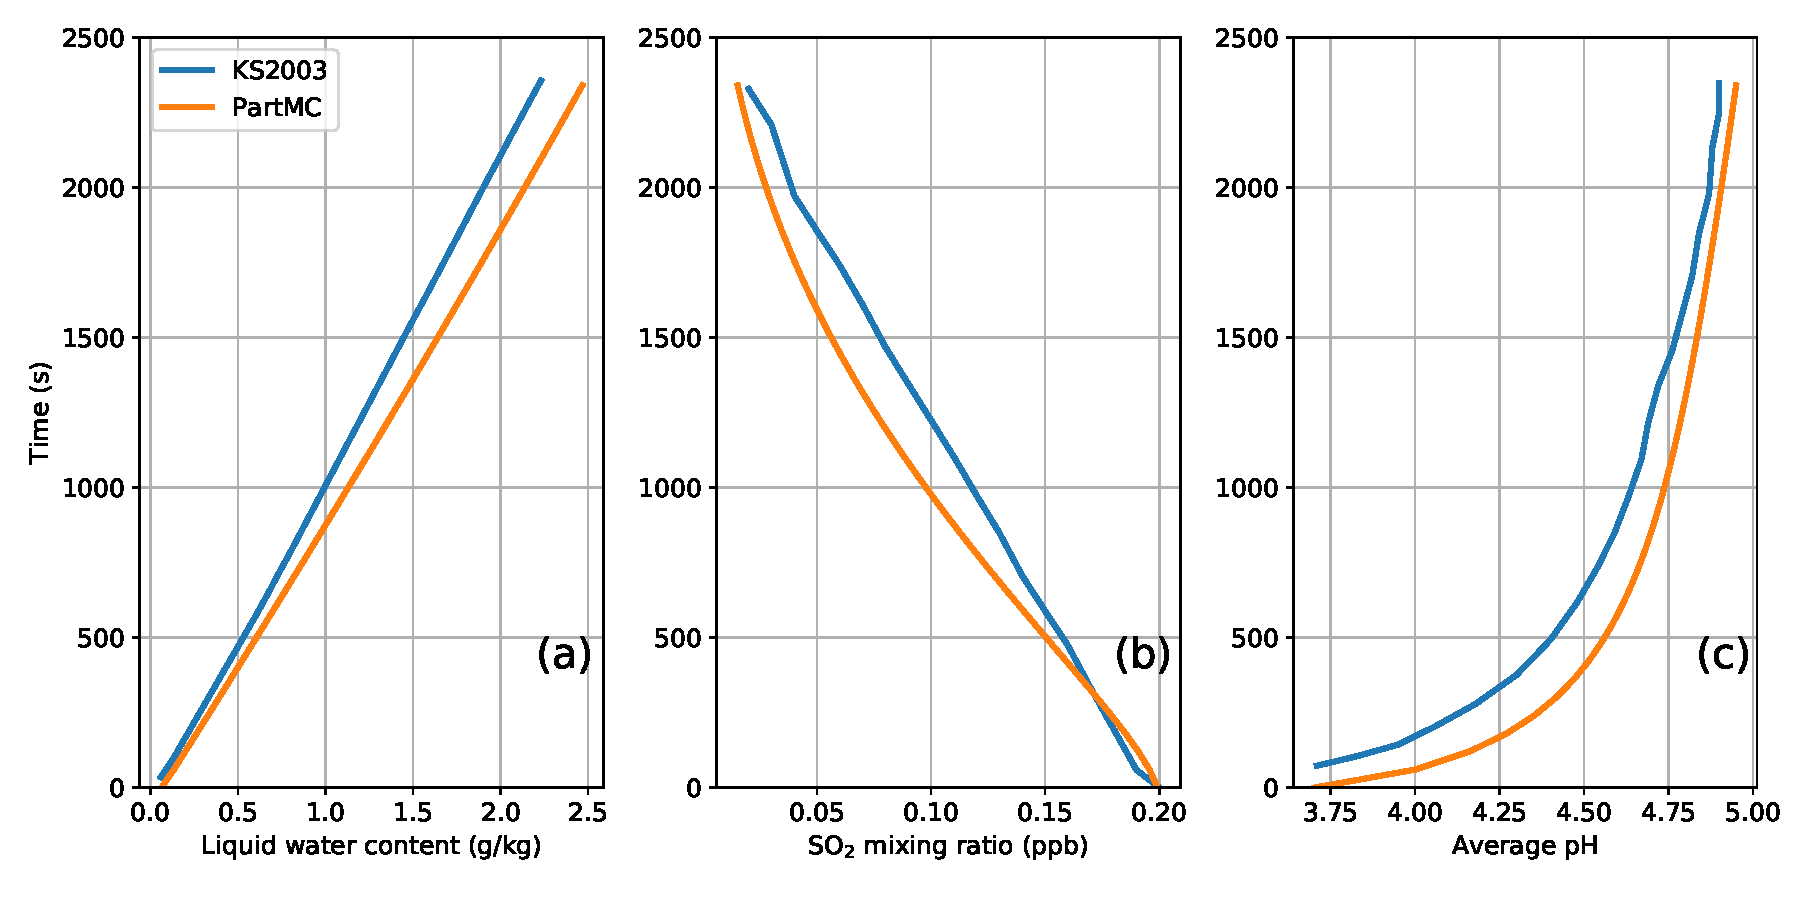
\includegraphics[scale=0.5]{chap2_figs/chap2_fig1_profile.pdf}
    \caption{Vertical profile differences of (a) liquid water content and (b) Gas $\rm SO_2$ concentration (c) Bulk pH between KS2003 and PartMC.}
    \label{chap2:ks2003}
\end{figure}

The simulated $\rm SO_2$(g) depleting rate is almost consistent between PartMC and KS2003 (Fig.~\ref{chap2:ks2003}(b)), with $\rm SO_2$(g) mixing ratio decreasing from 0.2 to 0.025~ppb after 40 minutes, indicating PartMC is capable of simulating of aqueous sulfate formation processes. The bulk acidity calculated by PartMC also shows similar profile with the models in KS2003 but with higher values (Fig.~\ref{chap2:ks2003}(c)). Considering the different simulation approaches, we are expecting the differences between bulk or size-binned based pH and our particle-resolved pH. 

Since sulfate aqueous formation pathways are highly acidity dependent, especially through $\rm O_3$, where reaction rates increase exponentially with increasing pH, the acidity differences imply noticeable changes in sulfate production. At the end of simulation, PartMC simulated sulfate concentration of 207 ppb, higher than the $\sim$175 in size-resolved models and $\sim$145 in bulk models. As explained in KS2003, the excess produced sulfate in the size-resolved models are found to be associated with higher simulated pH and more sulfate formed from $\rm O_3$ oxidation pathway. This explanation is still applicable for our current findings. 

In summary, this comparison simulation proved our particle-resolved aqueous model is capable of capturing the sulfate aqueous chemical processes. 
With more detail particle information, our particle-resolved approach may also provide more comprehensive understanding of different sulfate formation pathways, and this is explored in our next section. 
%\begin{figure}
\section{Contribution of different aqueous sulfate formation pathways}
\label{chap2.4}
This section explored the important factors for higher aqueous sulfate formation by analyzing the 243 aerosol populations in $P_{\rm ref}$.
Figure~\ref{chap2:ens_three} shows the sulfate mixing ratio in the ensemble scenarios, and values are categorized by different factors. There are clear sulfate formation separations between the cases with different ammonia gas mixing ratio, and cases with more sulfate production are associated with high ammonia environment. But this separation is not clear for other three considered factors, because cases with higher sulfate formation can be with all the three levels of temperature lapse rate, $\rm H_2O_2(g)$ and $\rm O_3(g)$mixing ratio. This phenomena indicates ammonia gas concentration is a determined factor for aqueous sulfate formation in current simulated scenarios. Next, we will look into the underlying theories.

\begin{figure}[ht]
    \centering 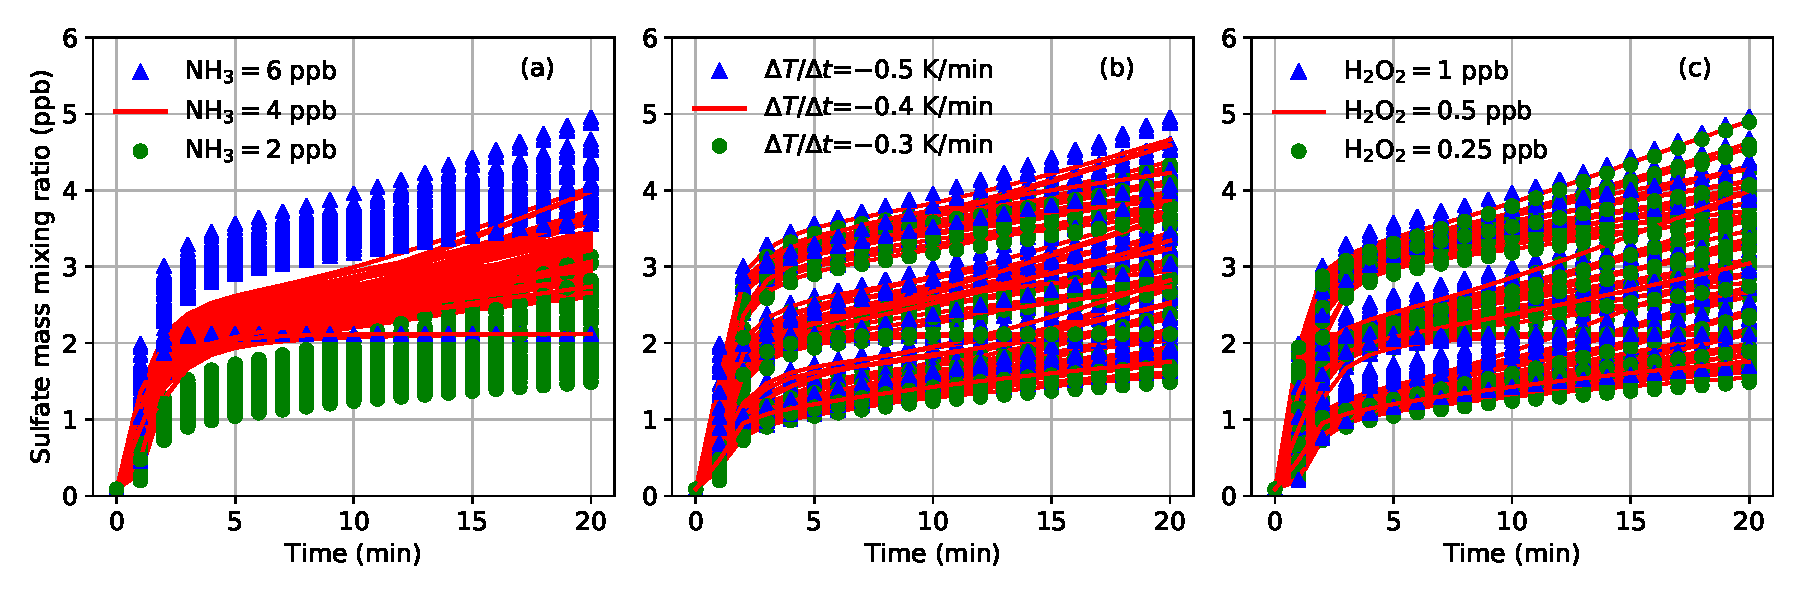
\includegraphics[scale=0.6]{chap2_figs/chap2_fig2_mono_ensemble.pdf}
    \caption{Sulfate time series categorized by four different settings in $P_{\rm ref}$: (a) initial $\rm NH_3(g)$ mixing ratio, (b) temperature lapse rate, (c) initial $\rm H_2O_2(g)$ mixing ratio, and (d) $\rm O_3(g)$ mixing ratio. The three colors and symbols are for the low, medium and high levels of each parameter.}
    \label{chap2:ens_three}
\end{figure}

The dissolved $\rm SO_2$ in cloud can appear in three S(IV) forms: $\rm SO_2\cdot H_2O$, $\rm HSO_3^-$ and $\rm SO_3^{2-}$. In this work, 
I analyzed four key oxidation pathways which transfer these S(IV) species to S(VI):
\begin{align}
\centering
    &\ce{HSO3^- + H2O2{(aq)} + H^+ -> SO4^{2-} + 2H^+ + [H2O](aq)}\\
    &\ce{HSO3^- + O3{(aq)} -> SO4^{2-} + H^+ + O2{(aq)}} \\
    &\ce{SO3^{2-} + O3{(aq)} -> SO4^{2-} + O2{(aq)}} \\
    &\ce{S(IV) + \frac{1}{2}O2 ->[TMI] S(VI)}
\label{eq:chem-eq}
\end{align}
This section will focus on the discussion of the first three oxidation pathways and transition pathway reaction (2.9) will be discussed in next section.

Figure~\ref{chap2:su-acidity} shows the relationship between sulfate mixing ratio and particle acidity at 3~\unit{min}. For the cases with same $\rm SO_2(g)$, sulfate mixing ratio is higher for those with higher $\rm NH_3(g)$. This is because of the higher pH values for these cases. Considering the cases with $\rm SO_2(g)$ of 5~\unit{ppb} and $\rm O_3(g)$ of 50~\unit{ppb}(the cases in the red boxes of Fig~\ref{chap2:su-acidity}), the only differences for these cases are $\rm NH_3(g)$ values. I found for all these three lapse rates, when $\rm NH_3(g)$ increased from 2 to 6~\unit{ppb}, pH increased from 5.0 to over 5.5 and sulfate mixing ratio increased from 1~\unit{ppb} to more than 2.5~\unit{ppb}. This is because the increased reaction rates of $\rm O_3$ pathways (Fig.~\ref{chap2:reac-rates}). In Fig.~\ref{chap2:reac-rates}, I also found for cases with 10~\unit{ppb} $\rm SO_2$, $\rm H_2O_2$ reaction rates are almost constant at all $\rm NH_3$ levels. The different responses of $\rm O_3$ and $\rm H_2O_2$ pathways are consistent with what \citet{Seinfeld2016} found. For $\rm O_3$ pathways, high pH leads to high S(IV) solubility and reaction rates increased. The reactions are self-limiting because the produced sulfate will increase acidity. For $\rm H_2O_2$ pathway, it is insensitive to pH because of the canceling effects between increased S(IV) concentration and reduced reaction constants. I also noticed for the cases with 2~\unit{ppb} $\rm SO_2$, reaction rates are smaller for those with higher $\rm NH_3$ and pH. These are the $\rm SO_2(g)$-limited cases and the less dissolved $\rm SO_2$ are responsible for this.  

\begin{figure}[ht]
    \centering 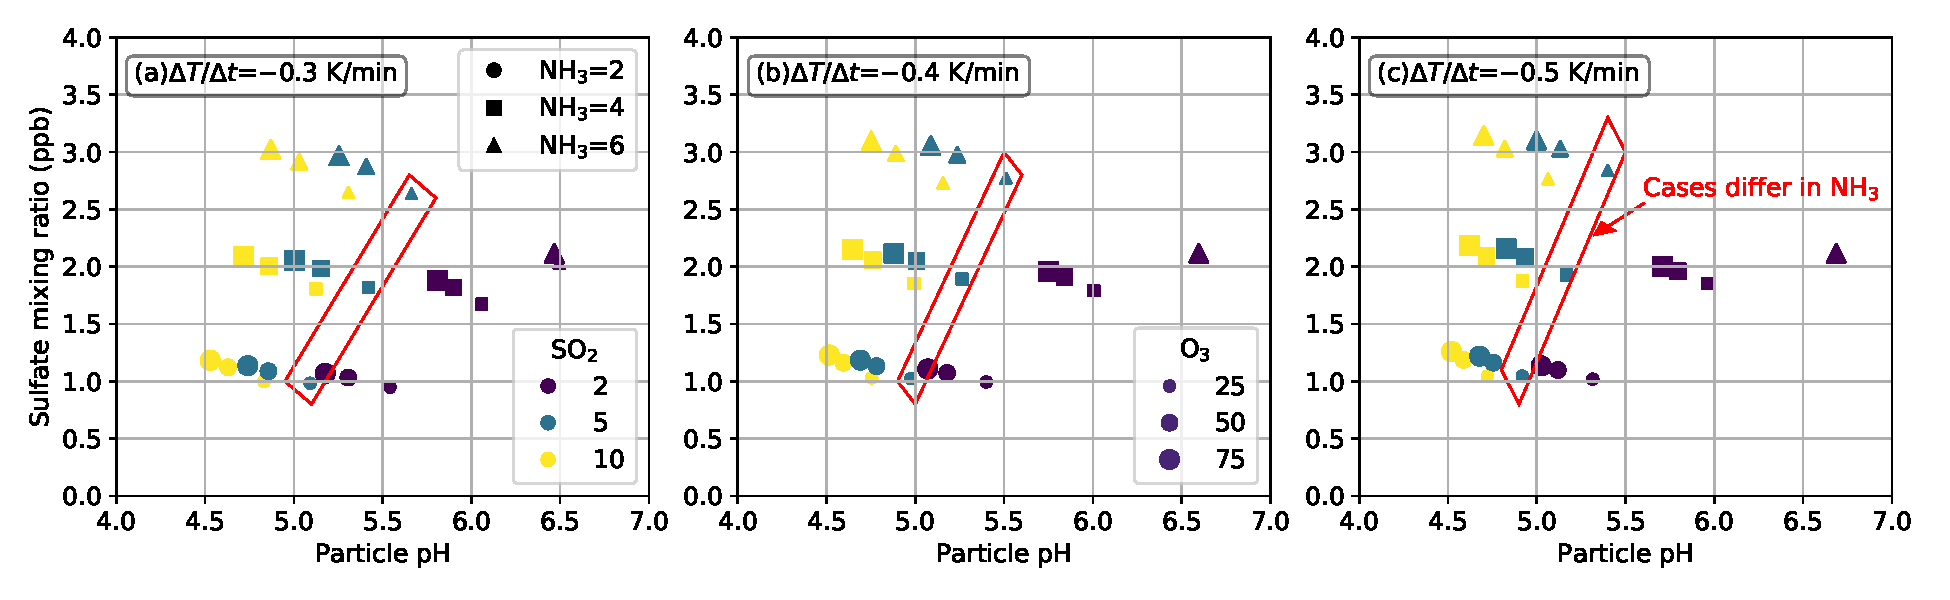
\includegraphics[scale=0.55]{chap2_figs/chap2_fig4_sulfate_pH_3min.pdf}
    \caption{Correlation between sulfate mixing ratio and acidity at 3~\unit{min}. (a) is for cases with temperature lapse rate of $-0.3$~\unit{K/min}. (b) is for cases with temperature lapse rate of $-0.4$~\unit{K/min}. (c) is for cases with temperature lapse rate of $-0.5$~\unit{K/min}. Symbols in the plots are colored by $\rm SO_2$(g) levels and symbol types are for $\rm NH_3$(g) levels. All the cases in the figure are with $\rm H_2O_2(g)$ = 0.5~\unit{ppb}. Red boxes are for the aerosol populations with only differences in $\rm NH_3(g)$ and are analyzed for detail in the text.}
    \label{chap2:su-acidity}
\end{figure}

As for the sensitivity to temperature, there is no significant differences for cases with different temperature lapse rates (Fig~\ref{chap2:reac-rates}). As \citet{Seinfeld2016} proposed, the effects of temperature on reaction rates are the balancing effects between two factors. For one hand, lower temperature leads to higher solubility and higher reactions rates. For the other hand, reaction constants decreased with lower temperature. Thus, when temperature changes, the behaviour of reactions rates are determined by which factor is dominant. 

\begin{figure}[ht]
    \centering 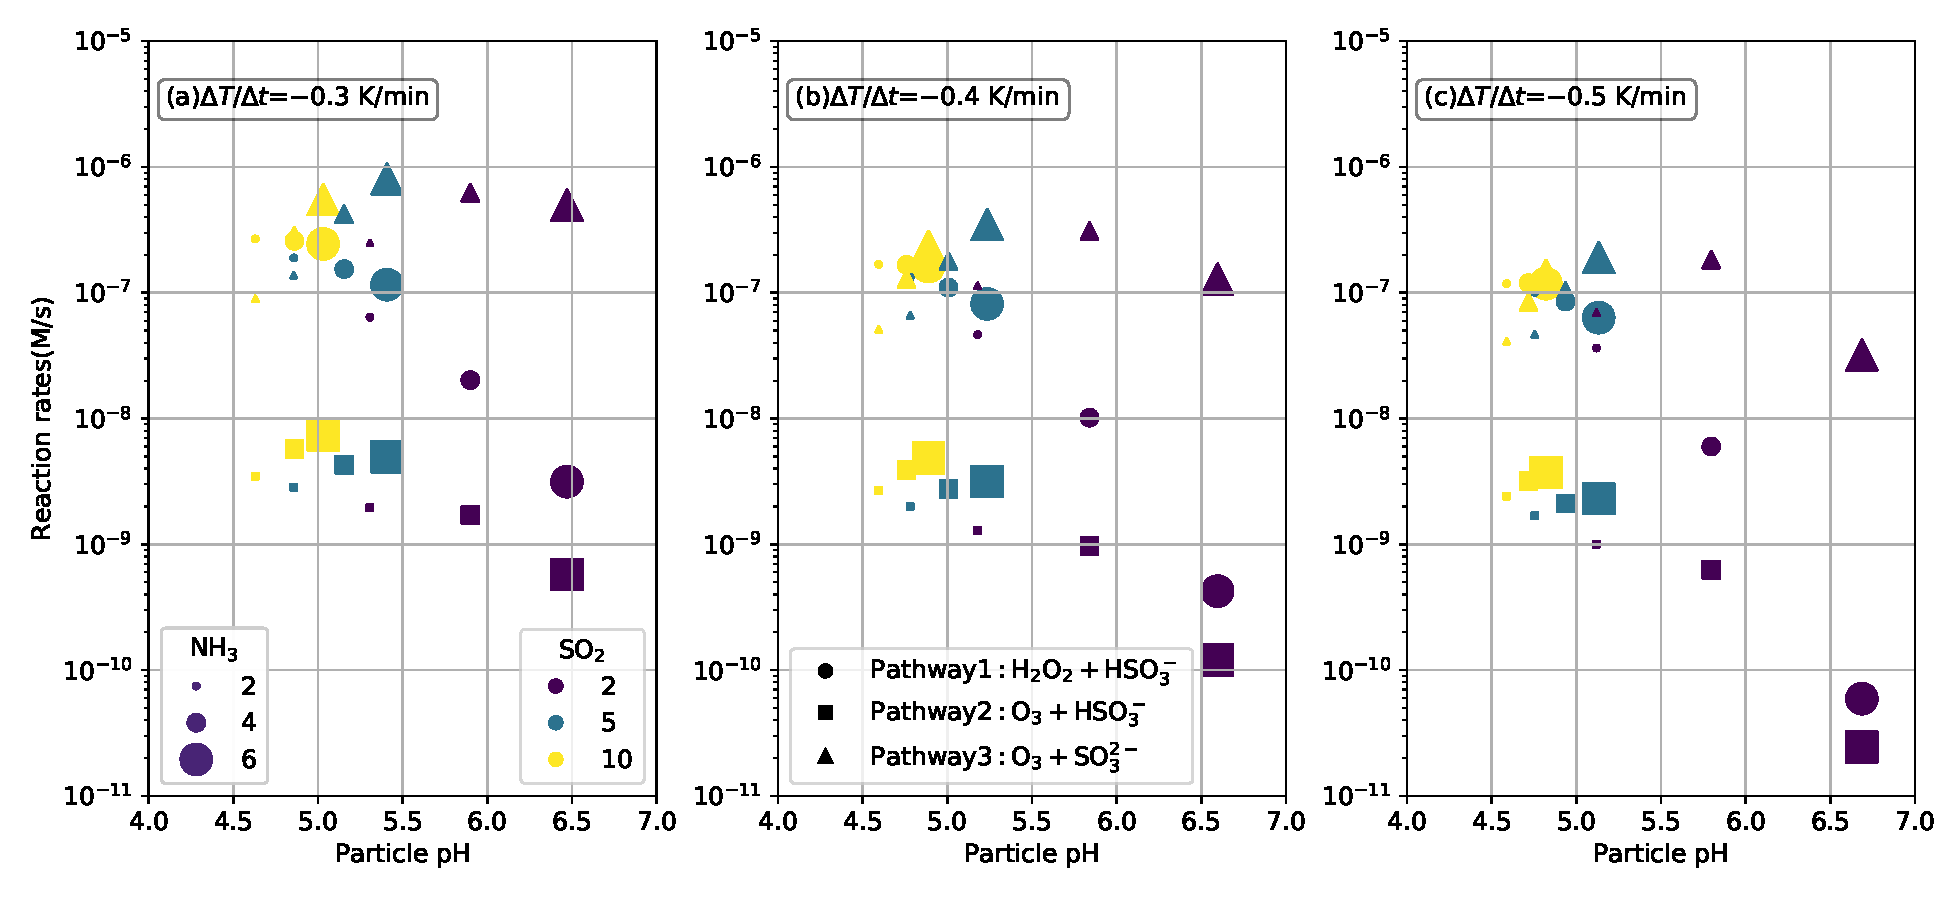
\includegraphics[scale=0.55]{chap2_figs/chap2_fig6_sulfate_pH.pdf}
    \caption{Correlation between aqueous sulfate formation pathway rates and particle acidity at 3~min. (a) is for cases with temperature lapse rate of $-0.3$~\unit{K/min}. (b) is for cases with temperature lapse rate of $-0.4$~\unit{K/min}. (c) is for cases with temperature lapse rate of $-0.5$~\unit{K/min}. Symbol types are for different oxidation pathways: circle is for $\rm H_2O_2+ HSO_3^-$, diamond is for $\rm O_3+ HSO_3^-$ and triangle is for $\rm O_3+ SO_3^{2-}$. Color is for $\rm SO_2(g)$ level and Symbol size represents $\rm NH_3(g)$ level. All the cases in the figure are with $\rm O_3(g)$ = 50~\unit{ppb} and $\rm H_2O_2(g)$ = 0.5~\unit{ppb}.}
    \label{chap2:reac-rates}
\end{figure}

%Detail statistics of the three pathways are further explored in Fig.~\ref{chap2:reac-rates}. Sulfate formation through $\rm H_2O_2+ HSO_3^-$ and $\rm O_3(aq)+ SO_3^{2-}$ pathways are 1--2 orders higher than $\rm O_3(aq) + HSO_3^-$. The higher rates of $\rm O_3+ SO_3^{2-}$ than $\rm O_3+ HSO_3^{-}$ can be explained by the different nucleophilic reactivity. The oxidation rates of $\rm HSO_3^-$ by $\rm H_2O_2(aq)$ and $\rm O_3(aq)$ increase rapidly with increasing $\rm SO_2$(g) mixing ratio. For the cases with 6~\unit{ppb} $\rm NH_3$(g), median reaction rates of $\rm H_2O_2(aq) + HSO_3^-$ jump from $10^{-9}$~\unit{M/s} at 2~\unit{ppb} $\rm SO_2$(g) to $10^{-7}$~\unit{M/s} at 10~\unit{ppb} $\rm SO_2$(g). But for oxidation of $\rm SO_3^{2-}$ by $\rm O_3(aq)$, the reaction rate and $\rm SO_2$(g) mixing ratio is negative correlated. That can explain why there is no strong correlation between $\rm SO_2$(g) mixing ratio and high sulfate formation rates. As for $\rm NH_3$(g), oxidation rates of $\rm HSO_3^-$ and $\rm SO_3^{2-}$ by $\rm O_3(aq)$ is higher at the cases with 6~\unit{ppb} $\rm NH_3$(g), and there is no clear change for $\rm H_2O_2(aq) + HSO_3^-$ at different $\rm NH_3$ levels. This is consistent with what we found the most sulfate formation cases are connected with high $\rm NH_3(g)$ cases. The only anomalous cases are for the aerosol populations with 2~\unit{ppb} $\rm NH_3(g)$, where the reaction rates decreased with increasing $\rm NH_3(g)$. This is the $\rm SO_2(g)$-limited cases we mentioned above. 

%\begin{figure}[ht]
%    \centering 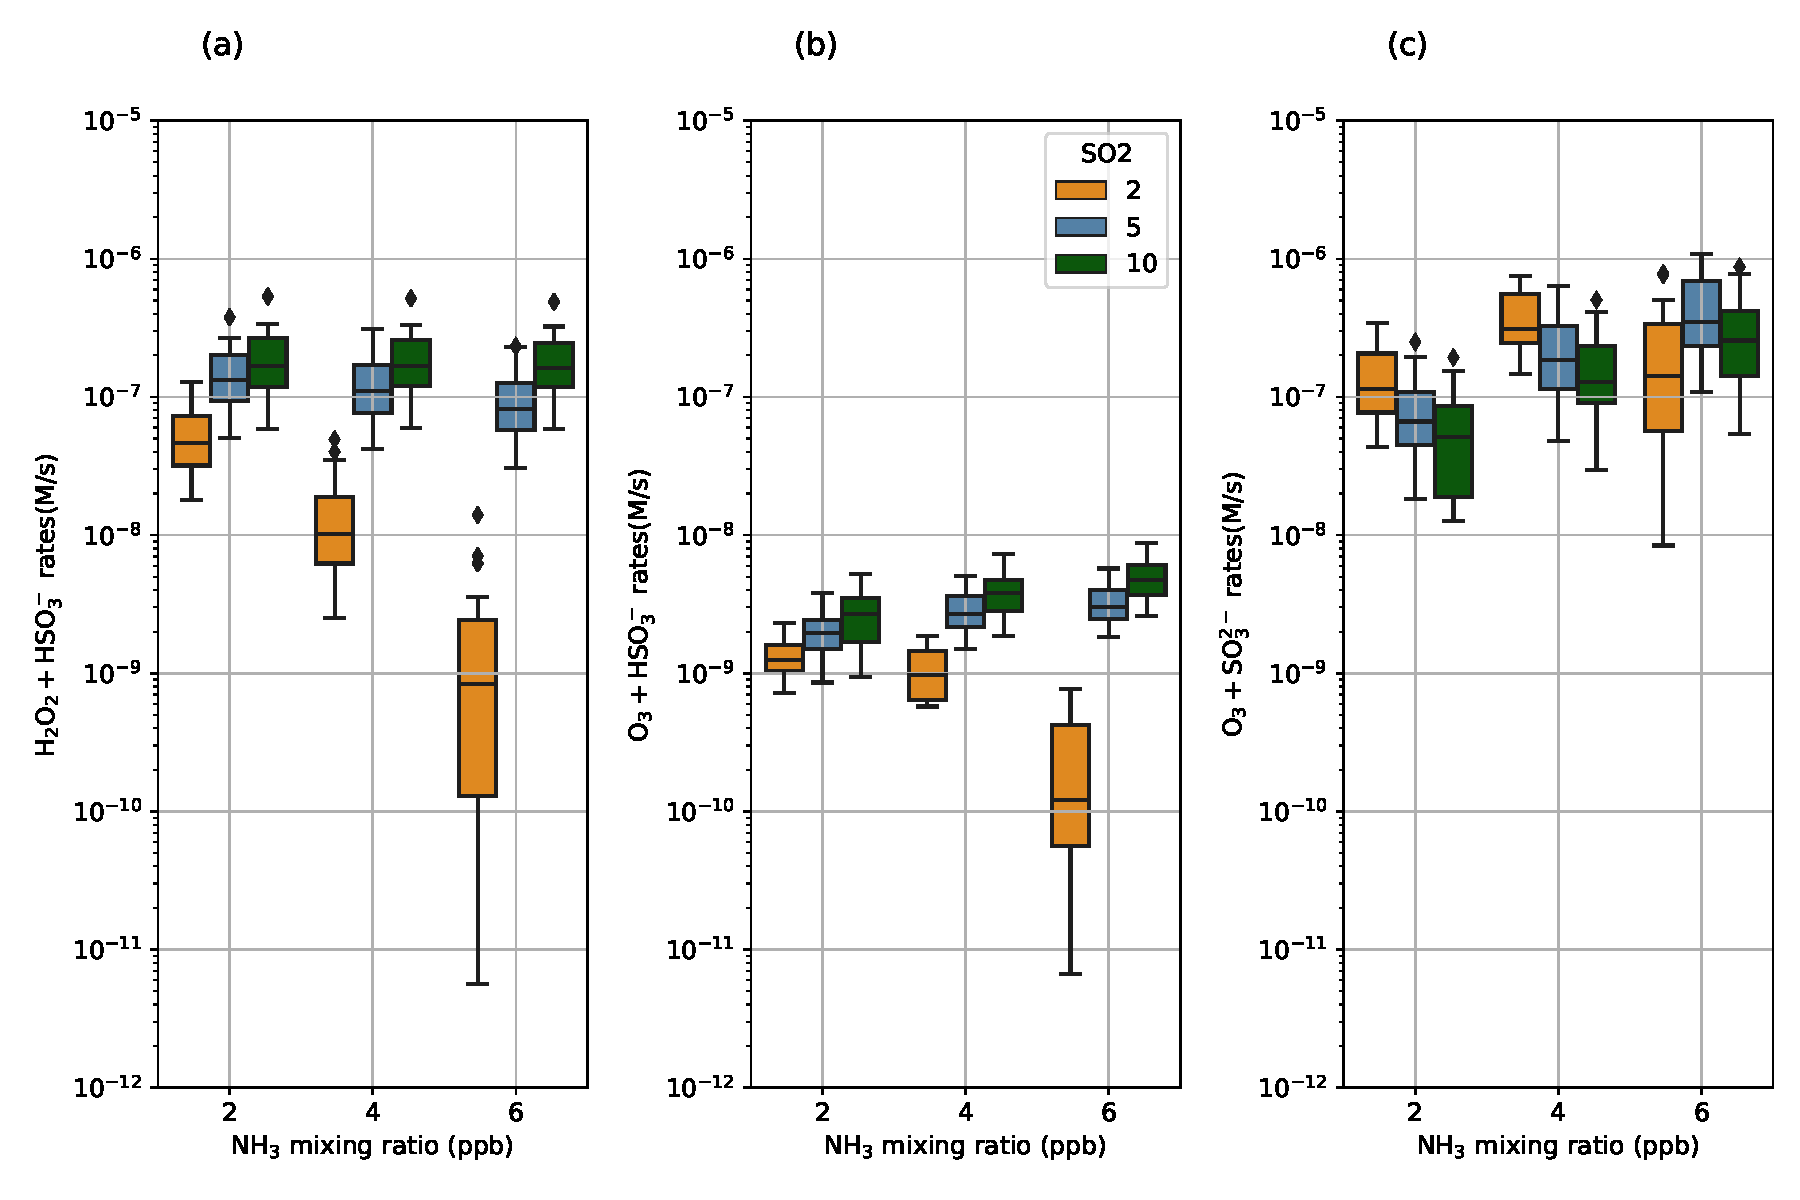
\includegraphics[scale=0.55]{chap2_figs/chap2_fig5_sulfate_rates_3min.pdf}
%    \caption{Statistics of three aqueous sulfate formation pathway rates:$\rm H_2O_2$ + $\rm HSO_3^-$(a), $\rm O_3$ + $\rm HSO_3^-$(b), $\rm O_3$ + $\rm SO_3^{2-}$. Cases are grouped by $\rm NH_3(g)$ and $\rm SO_2$.}
%    \label{chap2:rates-stats}
%\end{figure}

Based on analysis for the cases in $P_{\rm ref}$, I found the aqueous sulfate formation are most sensitive to the $\rm SO_2(g)$ and $\rm NH_3(g)$ mixing ratios. Cases with most sulfate formation were for the cases with high $\rm NH_3(g)$ values and this can be explained by the higher oxidation rates of $\rm SO_3^{2-}$ by $\rm O_3(aq)$. Cases with higher $\rm NH_3(g)$ but lower sulfate production were because of lower $\rm SO_2(g)$, and sulfate formation was $\rm SO_2(g)$-limited. I also concluded that our particle-resolved aqueous approach was capable of simulating the complex response of $\rm O_3$ and $\rm H_2O_2$ pathways to temperature and acidity changes. 

\section{Contribution of TMI pathways}
\label{chap2.5}
In this section, I will analyze the other 243 cases containing iron components in $P_{\rm TMI}$ and explore the contributions of TMI catalyzed reactions. Figure~\ref{chap2:iron-conc}(a) shows the time series of $\rm Fe^{2+}$, $\rm Fe^{3+}$ and OH(aq) mass concentration in the ensemble cases. $\rm Fe^{2+}$ varies between $10^{-11}$ and $10^{-7}$ and $\rm Fe^{3+}$ ranges between $10^{-7}$ and $10^{-6}$~\unit{M}, both are in the same order with the values in \citep{Deguillaume2005}. By adding TMI, the median sulfate mixing ratio in $P_{\rm TMI}$ significantly increased from 2~\unit{ppb} to 5~\unit{ppb}. Figure~\ref{chap2:iron-contri} further explores the contribution ratio changes of different aqueous sulfate pathways after adding TMI in the population. 

\begin{figure}[ht]
    \centering 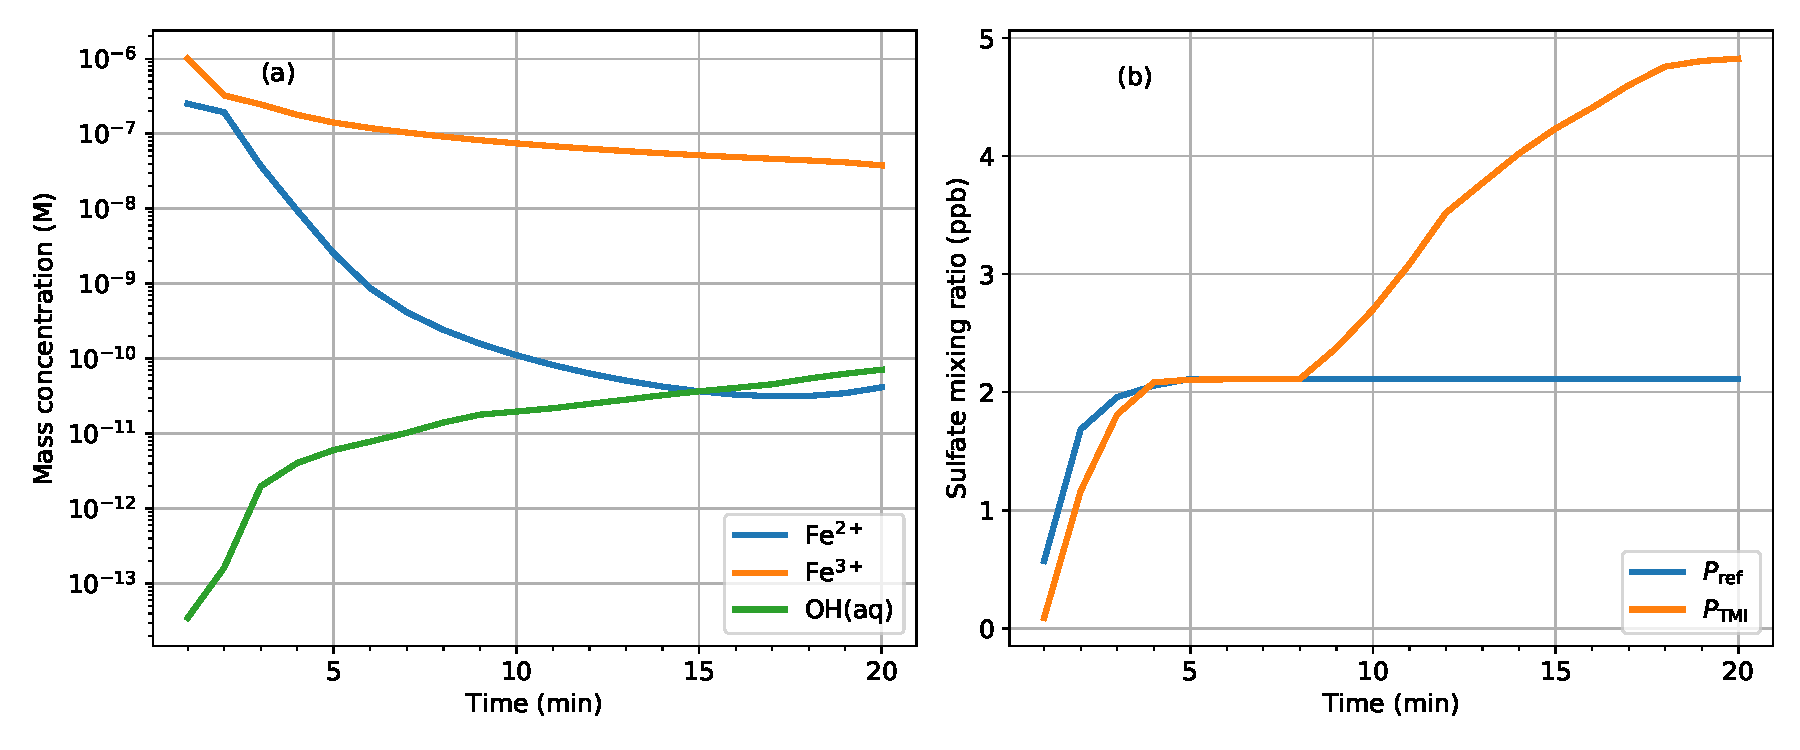
\includegraphics[scale=0.55]{chap2_figs/chap2_with_tmi_fixOH_mass.pdf}
    \caption{Time series of (a) $\rm Fe^{2+}$, $\rm Fe^{3+}$ and $\rm OH(aq)$ (b) Sulfate mixing ratio in $P_{\rm ref}$ and $P_{\rm TMI}$. Values are the median of all the ensemble cases in $P_{\rm TMI}$. }
    \label{chap2:iron-conc}
\end{figure}

Oxidation of $\rm HSO_3^-$ by $\rm O_3$ and $\rm H_2O_2$ are the dominant pathways for aqueous sulfate formation in $P_{\rm ref}$ (Fig.~\ref{chap2:iron-contri}(a)). These two pathways in total contributed to more than 90\% of sulfate formation along the simulation period, and there is minimum contribution of TMI pathways. But in $P_{\rm TMI}$, these two pathways are dominant at the first 2 minutes and sulfate formation through the reaction between $\rm SO_4^-$ and water is dominant afterwards (Fig.~\ref{chap2:iron-contri}(b)). I also noticed a remarkable contribution from TMI pathway after 4~\unit{min}, and the contribution ratio can be more than 20\% at the end of simulation. 

\begin{figure}[ht]
    \centering 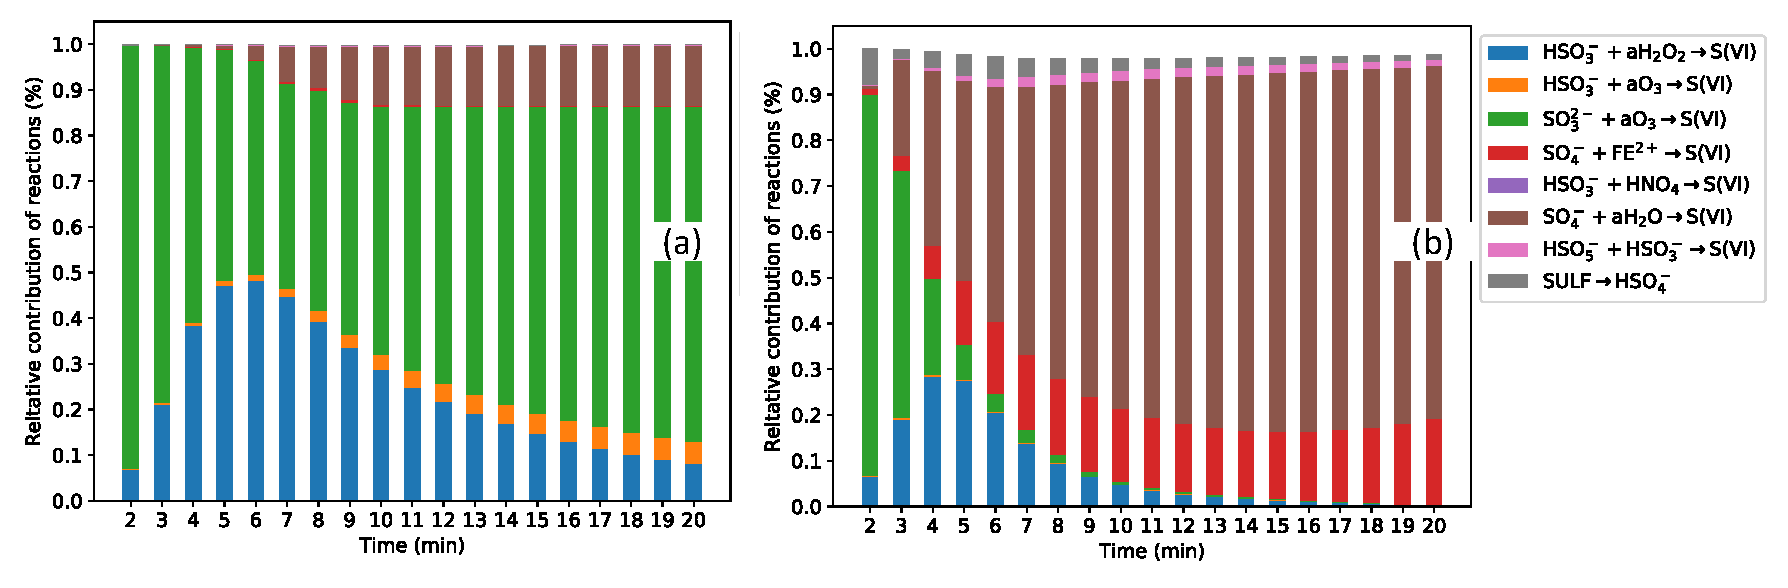
\includegraphics[scale=0.6]{chap2_figs/chap2-TMI_contri_factors.pdf}
    \caption{Mean contribution fraction of different sulfate formation pathways in (a)$P_{\rm ref}$ and (b)$P_{\rm TMI}$}
    \label{chap2:iron-contri}
\end{figure}

It is worth mention that gas OH emitted at a constant rate for the cases $P_{\rm TMI}$, while there is no emission in $P_{\rm ref}$. Based on current simulation setting, we can not distinguish the role of OH and TMI for the increased sulfate production rates in $P_{\rm TMI}$. Further simulations are needed to validate the current findings. But what we can still learn from current result is there exists some conditions where sulfate formation through TMI pathways can be important. 

\section{Conclusion}
\label{chap2.6}
In this work, I coupled particle-resolved PartMC-MOSAIC with a comprehensive aqueous chemistry 
module CAPRAM2.4 to investigate the role of different aqueous sulfate formation pathways. 
Model was evaluated by size-resolved and bulk aqueous models, and our model reproduced the similar $\rm SO_2$(g) and 
acidity profiles. 

I designed a reference scenario at various gas conditions to investigate the most efficient aqueous sulfate formation pathways.
I found cases with high $\rm NH_3(g)$ and $\rm SO_2(g)$ produced the most sulfate, and it can be explained by efficient oxidizing reactions between $\rm SO_3^{2-}$ and $\rm O_3(aq)$ because of the higher pH. Our particle-resolved aqueous model was proved to be capable of simulating the complicated responses of $\rm O_3$ and $\rm H_2O_2$ pathways to pH. Analysis of another ensemble scenario with TMI shows S(IV) reactions catalyzed by TMI can contribute up to 20\% of the sulfate production, and the ratio was consistent with the values found by \citet{alexander2009transition}. 

%%%Limitations%%%
Currently, I used monodisperse aerosol populations for analysis and in the future we should generalize our conclusions by more realistic aerosol populations, such as populations with several lognormal distribution. Also, I used rather simple way to represent TMI and OH(g) concentrations. Since Fe from different sources have different solubility \citep{desboeufs2005dissolution}, it would be better to connect Fe soluble fraction and OH(g) emitting rates with aerosol sources to confirm the conditions most favorable for TMI-catalyzed reactions. 

\backmatter
\renewcommand{\bibname}{References}
\bibliographystyle{copernicus}
\bibliography{thesis_ref}
\end{document}

\appendix
% Reset the algorithm counter
\setcounter{algorithm}{0}

\chapter{Appendix to Chapter~\ref{chap2:mon}}
\label{tab:capram}
\section{List of aqueous reactions coupled to PartMC-MOSAIC}
This appendix shows the thermodynamic and kinetic data for the aqueous chemistry reactions 
coupled with PartMC-MOSAIC. It is based on the reduced CAPRAM 2.4 mechanism, 
and the full mecahnism can refer to \citet{Ervens2003}.
Table~\ref{Henry} lists the coefficients for Henry's Law.
%%%%%%%Table A1%%%%%%%%
\begin{table}[ht]
\centering
\caption{Henry's Law coefficients} \centering
\label{Henry}
\begin{threeparttable}
\begin{tabular}{ c l c c}
\toprule Henry's Law & Equilibrium & $K_{298}$ (M $\rm atm^{-1}$)$^*$& $-\Delta H/R$ (K) \\ 
\midrule
H1  & \ce{CO_2{(\rm g)}  <=> CO_2{(\rm aq)}} & 3.1$\times 10^{-2}$& 2423 \\ 
H2 & \ce{O_3{(\rm g)} <=> O_3{(\rm aq)}} &1.14 $\times 10^{-2}$ & 2300 \\ 
H3  & \ce{HO_2{(\rm g)}  <=> HO_2{(\rm aq)}} & 9.0$\times 10^{3}$& 0 \\ 
H4  & \ce{OH{(\rm g)}  <=> OH{(\rm aq)}} & 25 & 5280 \\ 
H5  & \ce{H_2O_2{(\rm g)} <=> H_2O_2{(\rm aq)}} &1.02 $\times 10^{5}$ & 6340 \\ 
H6  &\ce{NO_2{(\rm g)} <=> NO_2{(\rm aq)}} &1.2 $\times 10^{-2}$ & 1263\\
H7  &\ce{HONO{(\rm g)} <=> HONO{(\rm aq)}} & 49 & 4880\\
H8  & \ce{HNO_3{(\rm g)} <=> NO_3^- + H^+} &4.62 $\times 10^{6}$& 10500\\
H9  &\ce{NO_3{(\rm g)} <=> NO_3{(\rm aq)}} &6 $\times 10^{-1}$ & 0\\ 
H10  &\ce{N_2O_5{(\rm g)} <=> N_2O_5{(\rm aq)}} &1.4 $\times 10^{0}$ & 0\\ 
H11 & \ce{NH_3{(\rm g)}  <=> NH_3{(\rm aq)}} & 60.7 & 3920 \\ 
H12 & \ce{HCL{(\rm g)}  <=> CL^{-} + H^{+}} & 1.89$\times 10^6$ & 8910 \\ 
H13 & \ce{HCHO{(\rm g)}  <=> HCHO{(\rm aq)}} & 2.5 & 7216 \\ 
H14 & \ce{ORA{1}{(\rm g)}  <=> ORA{1}{(\rm aq)}} & 5.53$\times 10^3$ & 5630 \\ 
H15 &\ce{SO2{(\rm g)}  <=> SO2{(\rm aq)}} & 1.24 & 3247  \\ 
H16 &\ce{OP{1}{(\rm g)}  <=> OP{1}{(\rm aq)}} & 310 & 5607  \\ 
H17 &\ce{ORA{2}{(\rm g)}  <=> ORA{2}{(\rm aq)}} & 5.5$\times 10^3$ & 5890  \\ 
H18 &\ce{MO{2}{(\rm g)}  <=> MO{2}{(\rm aq)}} & 310 & 5607  \\ 
H19 &\ce{ETHPX{(\rm g)}  <=> ETHPX{(\rm aq)}} & 340 & 87  \\ 
H20 &\ce{ETOH{(\rm g)}  <=> ETOH{(\rm aq)}} & 190 & 6290  \\ 
H21 &\ce{CH{3}OH{(\rm g)}  <=> CH{3}OH{(\rm aq)}} & 220 & 5390  \\ 
H22 &\ce{ALD{(\rm g)}  <=> ALD{(\rm aq)}} & 4.8 & 6254  \\ 
H23 &\ce{BR{2}{(\rm g)}  <=> BR{2}{(\rm aq)}} & 0.758 & 3800  \\ 
H24 &\ce{CL{2}{(\rm g)}  <=> CL{2}{(\rm aq)}} & 9.15$\times 10^{-2}$ & 2490  \\ 
H25 &\ce{SULF{(\rm g)}  <=> HSO_4^- + H^{+}} & 8.7$\times10^{14}$ & 0 \\
H26 &\ce{HNO4{(\rm g)}  <=> HNO4{(\rm aq)}} &3$\times 10^4$& 0 \\ 
H27 &\ce{ACO3{(\rm g)}  <=> ACO3{(\rm aq)}} &6.69$\times 10^2$& 5893 \\ 
H28 &\ce{GLY{(\rm g)}  <=> GLY{(\rm aq)}} &1.40& 0 \\ 
H29 &\ce{[O_2]^{**}{(\rm g)}  <=> O_2{(\rm aq)}} &1.3$\times 10^{-3}$& 1700 \\ 
\bottomrule
\end{tabular}
\end{threeparttable}
\end{table}

% Table continued on next page
\addtocounter{table}{-1}
\begin{table}[ht]
\centering
\begin{threeparttable}
\caption{Continued.}
\begin{tabular}{ c l c c}
\toprule Henry's Law & Equilibrium & $K_{298}$ (M $\rm atm^{-1}$) & $-\Delta H/R$ (K) \\ 
\midrule
H30 &\ce{CLNO2{(\rm g)}  <=> CLNO2{(\rm aq)}} &0.024& 0.0 \\ 
H31 &\ce{BRNO2{(\rm g)}  <=> BRNO2{(\rm aq)}} & 0.3 & 0.0 \\ 
H32 &\ce{BRCL{(\rm g)}  <=> BRCL{(\rm aq)}} &0.94& 0.0 \\ 
H33 &\ce{NO{(\rm g)}  <=> NO{(\rm aq)}} &1.9$\times 10^{-3}$& 0.0 \\ 
\bottomrule
%\vspace*{5mm}
\end{tabular}
\begin{tablenotes}[para,flushleft]
      \small
      \item $*$: $K = K_{298} {\rm exp}(-\frac{\Delta H}{R}(\frac{1}{T}- \frac{1}{298}))$\\
      \item $**$: Specie with square bracket indicates its concentration is constant. 
\end{tablenotes}
\end{threeparttable}
\end{table}

Table~\ref{aq-ox} lists the coefficients for aqueous chemical reactions. 
%%%%%%Table A2%%%%%%%%%%%%
\begin{table}[ht]
\centering
\caption{Aqueous chemical reactions} \centering
\label{aq-ox}
\begin{threeparttable}
\begin{tabular}{ c l c c}
\toprule Aqueous chemistry & Reaction & $ K_{298}$ (${\rm M}^{-n}$ $\rm s^{-1}$) & $-E/R$ (K) \\ 
\midrule
A1 & \ce{FEOH^{2+} -> FE^{2+} + OH(\rm aq)} & 4.76$\times 10^{-3}$ & 2.20 \\
A2 & \ce{NO3^{-} -> NO2(\rm aq) + OH(\rm aq) + OH^{-}}& 4.57$\times 10^{-7}$ & 2.59 \\
A3 & \ce{H2O2(\rm aq) -> OH(\rm aq) + OH(\rm aq)} & 7.64$\times 10^{-6}$ & 2.46 \\
A4 & \ce{FEC2(O4)_2^{-} -> FE^{2+} + C2O4^{2-} + CO2(\rm aq) + CO2^{-}} &2.47 $\times 10^{-2}$& 1.96 \\
A5 & \ce{H2O2(\rm aq) + FE^{2+} -> FE^{3+} + OH(\rm aq) + OH^{-}} & 50.0 & 0.0 \\
A6 & \ce{H2O2(\rm aq) + Cu^+ -> Cu^{2+} + OH(\rm aq) + OH^-} & 7000.0 & 0.0 \\
A7 & \ce{O2^- + FE^{3+} -> FE^{2+} + O2(\rm aq)} & 1.5$\times 10^8$ & 0.0 \\
A8 & \ce{HO2(\rm aq) + FE(OH)^{2+} -> FE^{2+} + O2(\rm aq) + [H2O](\rm aq)} &1.3$\times 10^5$& 0.0 \\
A9 & \ce{O2^{-}(\rm aq) + FE(OH)^{2+} -> FE^{2+} + O_2(\rm aq) + OH^-} & 1.5$\times 10^8$ & 0.0 \\
A10 & \ce{O2^- + FE^{2+} -> FE^{3+} + H2O2(aq) + 2OH^- - 2[H2O](aq)} & 1.0$\times 10^7$ & 0.0 \\
A11 & \ce{HO2(aq) + FE^{2+} -> FE^{3+} + H2O2(aq) + 2OH^- -2[H2O](aq)} & 1.2$\times 10^6$& --5050.0 \\
A12 & \ce{OH(aq) + FE^{2+} -> FE(OH)^{2+}} & 4.3$\times 10^8$ & --1100 \\
A13 & \ce{O2^- + Cu^+ -> Cu^{2+} + H2O2(aq) + 2OH^- -2[H2O](aq)} & 1.0$\times 10^{10}$& 0.0 \\
A14 & \ce{HO2(aq) + Cu^+ -> Cu^{2+} + H2O2(aq) + OH^- -[H2O](aq)} & 2.3$\times 10^9$& 0.0 \\
A15 & \ce{HO2(aq) + Cu^{2+} -> Cu^+ + O2(aq) + H^+} & 1.0$\times 10^8$ & 0.0 \\
A16 & \ce{O2^- + Cu^{2+} -> Cu^+ O2(aq)} & 8$\times 10^9$ & 0.0 \\
A17 & \ce{FE^{3+} + Cu^+ ->= FE^{2+} + Cu^{2+}} & 1.3$\times 10^7$ & 0.0\\
A18 & \ce{FE(OH)^{2+} + Cu^+ -> FE^{2+} + Cu^{2+} + OH^-} & 1.3$\times 10^7$ & 0.0 \\
A19 & \ce{O3(\rm aq) + O2^- -> O3^- + O2(rm aq)} & 1.5$\times 10^9$ & 0.0 \\
A20 & \ce{HO3(aq) -> OH(\rm aq) + O2(\rm aq)} & 330.0 & --4500.0 \\
A21 & \ce{H2O2{(\rm aq)} + OH{(\rm aq)} -> HO_2{(\rm aq)} + H_2O} &3.0 $\times 10^{7}$& --1680 \\  
A22 & \ce{HSO3^- + OH{(\rm aq)} -> SO3^{-} + H2O}&2.7 $\times 10^{9}$& 0 \\ 
A23 & \ce{Cu^+ + O2(\rm aq) -> Cu^{2+} + O2^-} & 4.6$\times 10^5$& 0.0 \\
A24 & \ce{FE^{2+} + O3(aq) -> FEO^{2+} + O2(aq)} & 8.2$\times 10^5$ & --4690.0 \\
A25 & \ce{FEO^{2+} + Cl^- -> FE^{3+} + CLOH^- + OH^- - [H2O](aq)} & 100.0 & 0.0 \\
\bottomrule
\end{tabular}
\end{threeparttable}
\end{table}

% Table continued on next page
\addtocounter{table}{-1}
\begin{table}[ht]
\centering
\begin{threeparttable}
\caption{Continued.}
\begin{tabular}{ c l c c}
\toprule Aqueous chemistry & Reaction & $ K_{298}$ (${\rm M}^{-n}$ $\rm s^{-1}$) & $-E/R$ (K) \\ 
\midrule
A26 & \ce{FEO^{2+} + FE^{2+} -> 2FE^{3+} + 2OH^-} & 7.2$\times 10^4$ & --842.0 \\
A27 & \ce{N2O5(aq) -> NO2^+ + NO3^-} & 1.0$\times 10^9$ & 0.0 \\
A28 & \ce{NO2^+ + [H2O](aq) -> NO3^- + H^+ + SO3^-} & 8.9$\times 10^7$ & 0.0 \\
A29 & \ce{NO3(aq) + HSO3^-  -> NO3^- + H^+ + SO3^-} &1.3 $\times 10^{9}$& --2000.0\\ 
A30 & \ce{NO3(aq) + SO4^{2-}  -> NO3^- + SO4^-} & 1.0 $\times 10^{5}$& 0.0\\
A31 & \ce{NO4^-  -> NO2^- + O2{\rm (aq)}} & 4.5$\times10^{-2}$ & 0.0 \\ 
A32 & \ce{HNO4{(aq)} + HSO3^- -> HSO4^- + H^+ + NO3^-} &3.3 $\times 10^{5}$& 0.0 \\ 
A33 & \ce{NO2^+ + Cl^- -> CLNO2(aq)} & 1.0$\times 10^{10}$& 0.0 \\
A34 & \ce{NO2^+ + Br^- -> BRNO2(aq)} & 1.0$\times 10^{10}$& 0.0 \\
A35 & \ce{CLNO2(aq) + Br^- -> NO2^- + BRCL(aq)} & 5.0$\times 10^6$ & 0.0 \\
A36 & \ce{BRNO2(aq) + Br^- -> BR2(aq) + NO2^-} & 2.55$\times 10^4$ & 0.0 \\
A37 & \ce{BRNO2(aq) + Cl^- -> NO2^- + BrCl(aq)} & 10.0 & 0.0 \\
A38 & \ce{HMS^- + OH(aq) -> CHOHSO3^- + [H2O](aq)} & 3.0$\times 10^8$ & 0.0 \\
A39 & \ce{O2CHOHSO3^- + O2(aq) -> O2CHOHSO3^-} & 2.6$\times 10^9$& 0.0 \\
A40 & \ce{O2CHOHSO3^- -> HO2(aq) + CHOSO3^-} & 1.7$\times 10^4$ & 0.0 \\
A41 & \ce{O2CHOHSO3^- -> O2CHO(aq) + HSO3^-} & 7$\times 10^3$ & 0.0 \\
A42 & \ce{CHOSO3^- + [H2O](aq) -> HSO3^- + ORA{1}(aq)} & 1.26$\times 10^{-2}$ & 0.0 \\
A43 & \ce{O2CHO(aq) + [H2O](aq) -> ORA{1}(aq) + HO2(aq)} & 44.32 & 0.0 \\
A44 & \ce{HSO3^- + H2O2{(aq)} + H^+ -> SO4^{2-} + 2H^+ + [H2O](aq)} &7.2 $\times 10^{7}$& $-$4000.0\\ 
A45 & \ce{HSO3^- + O3{(aq)} -> SO4^{2-} + H^+ + O2{(aq)}} &3.7 $\times 10^{5}$& $-$5530.0 \\ 
A46 & \ce{SO3^{2-} + O3{(aq)} -> SO4^{2-} + O2{(aq)}} &1.5 $\times 10^{9}$& $-$5280.0 \\ 
A47 & \ce{SO5^{-} + FE^{2+} -> HSO5^- + FEOH^{2+}} & 2.65 $\times 10^7$ & -- 5809.0 \\
A48 & \ce{HSO5^- + FE^{2+} -> SO4^- + FEOH^{2+}} & 3.0$\times 10^4$ & 0.0 \\
A49 & \ce{FE^{2+} + SO4^- -> FEOH^{2+} + SO4^{2-} + H^+} & 4.6$\times 10^9$ & 2165.0 \\
A50 & \ce{SO5^- + SO5^- -> SO4^- + SO4^- + O2(aq)} & 2.2 $\times 10^8$ & --2600.0 \\ 
A51 & \ce{SO5^- + HO2{(aq)} -> SO5O2H^-} & 1.7$\times 10^9$ & 0.0 \\
A52 & \ce{SO5O2^{2-} -> HSO5^- + O2(aq) + OH^- -[H2O](aq)} & 1.2$\times 10^3$ & 0.0 \\
A53 & \ce{SO3^- + O2{(\rm aq)} -> SO5^-} & 2.5$\times10^9$ & 0.0 \\ 
A54 & \ce{SO4^- + [H_2O](aq) -> SO4^{2-} + OH{(\rm aq)} + H^+} & 11.0 & -1110.0 \\
A55 & \ce{HSO5^- + HSO3^- + H^+ -> 2SO4^{2-} + 3H^+ } & 7.14$\times 10^6$& 0.0 \\
A56 & \ce{CH3OH(aq) + OH(aq) -> CH2OH(aq) + [H2O](aq)} & 1.0$\times 10^9$ & 0.0 \\
A57 & \ce{CH2OH(aq) + O2(aq) -> O2CH2OH(aq)} & 2 $\times 10^9$ & 0.0 \\
A58 & \ce{O2CH2OH(aq) + O2CH2OH(aq) -> CH2OH(aq) + O2(aq) + aHCHO} & 1.05$\times 10^9$ & 0.0 \\
A59 & \ce{ETOH(aq) + OH(aq) -> CH3CHOH(aq) + [H2O](aq)} & 1.9$\times 10^9$ & 0.0 \\
A60 & \ce{CH3CHOH(aq) + O2(aq) -> O2CH3CHOH(aq)} & 2.0$\times 10^9$ & 0.0 \\
A61 & \ce{O2CH3CHOH(aq) + ALD(aq) -> HO2(aq)} & 52.0 & --7217.0 \\
A62 & \ce{CH2OH2(aq) + OH(aq) -> CHOH2(aq) + [H2O](aq)} & 1.0 $\times 10^9$ & --1020.0 \\
A63 & \ce{CHOH2(aq) + O2(aq) -> HO2(aq) + ORAQ1(aq)} & 2.0$\times 10^9$ & 0.0 \\
A64 & \ce{CH3CHOH2(aq) + OH(aq) -> CH3COH2(aq) + [H2O](aq)} & 1.2$\times 10^9$ & 0.0 \\
A65 & \ce{ALD(aq) + OH(aq) -> CH3CO(aq) + [H2O](aq)} & 3.6$\times 10^9$ & 0.0 \\
A66 & \ce{ORA{1}(aq) + OH(aq) -> CO2H(aq) + [H2O](aq)} & 1.3$\times 10^8$ & $-1000.0$ \\
A67 & \ce{HCOO^- + OH(aq) -> CO2H(aq) + OH^-} & 3.2 $\times 10^9$ & $-1000.0$ \\
A68 & \ce{ORA2(aq) + OH(aq) -> CH2COOH(aq) + [H2O](aq)} & 1.5$\times 10^7$ & $-1330.0$ \\
A69 & \ce{MCOO^- + OH(aq) -> CH2COO^- + [H2O](aq)} & 1.5$\times 10^7$ & --1800.0 \\
A70 & \ce{CH2COOH(aq) + O2(aq) -> ACO3(aq)} & 1.7 $\times 10^9$ & 0.0 \\
A71 & \ce{MO2(aq) + MO2(aq) -> CH3OH(aq) + HCHO(aq) + O2(aq)} & 7.4$\times 10^7$ & 0.0 \\
A72 & \ce{MO2(aq) + MO2(aq) -> Ch3O(aq) + CH3O(aq) + O2(aq)} & 3.6$\times 10^7$ & --2200.0 \\
A73 & \ce{ACO3(aq) + ACO3(aq) -> 2MO2(aq) + 2CO2(aq) + O2(aq)} & 1.5$\times 10^8$ & 0.0 \\
A74 & \ce{MO2(aq) + HSO3^- -> OP1(aq) + SO3^-} & 5.0$\times 10^5$ & 0.0\\
\bottomrule
%\vspace*{5mm}
\end{tabular}
\end{threeparttable}
\end{table}

% Table continued on next page
\addtocounter{table}{-1}
\begin{table}[ht]
\centering
\begin{threeparttable}
\caption{Continued.}
\begin{tabular}{ c l c c}
\toprule Aqueous chemistry & Reaction & $ K_{298}$ (${\rm M}^{-n}$ $\rm s^{-1}$) & $-E/R$ (K) \\ 
\midrule
A75 & \ce{ETHPX(aq) + ETHPX(aq) -> CH3CH2O(aq) + CH3CH2O(aq) + O2(aq)} & 1.0$\times 10^8$ & 750.0 \\
A76 & \ce{CH3CH2O(aq) -> CH3CHOH(aq)} & 1.0$\times 10^6$ & 0.0 \\
A77 & \ce{OH(aq) + HC2O4^- -> C2O4^- + [H2O](aq)} & 3.2$\times 10^7$ & 0.0 \\
A78 & \ce{OH(aq) + C2O4^{2-} -> OH^- + C2O4^-} & 5.3$\times 10^6$ & 0.0 \\
A79 & \ce{C2O4^- + O2(aq) -> CO2(aq) + O2^- + CO2(aq)} & 2$\times 10^9$ & 0.0 \\
A80 & \ce{OH(aq) + CHOH2CHOH2(aq) -> COH2CHOH2(aq) + [H2O](aq)} &1.1$\times 10^9$  & --1516.0 \\
A81 & \ce{COH2CHOH2(aq) + O2(aq) -> aO2COH2CHOH2(aq)} & 1.38$\times 10^9$ & 0.0 \\
A82 & \ce{O2COH2CHOH2(aq) -> HO2(aq) + CHOH2COOH(aq)} & 2$\times 10^9$ & 0.0\\
A83 & \ce{HO(aq) + CHOH2COOH(aq)  ->  COH2COOH(aq) + [H2O](aq)} & 1.1$\times 10^9$& --1516.0 \\
A84 & \ce{COH2COOH(aq) + O2(aq) -> O2COH2COOH(aq)} & 2.0$\times 10^9$ & 0.0 \\
A85 & \ce{O2COH2COOH(aq)  -> HO2(aq) + H2C2O4(aq)} & 2.0$\times 10^9$ & 0.0 \\
A86 & \ce{CH3COH2(aq) + O2(aq) -> CH3COH2OO(aq)} & 2.0$\times 10^9$& 0.0 \\
A87 & \ce{CH3COH2OO(aq) -> H^+ + H^+ + MCOO^- + O2^-} & 1.0$\times 10^5$ & 0.0\\
A88 & \ce{CH3O(aq) -> CH2OH(aq)} & 1.0$\times 10^6$ & 0.0 \\
A89 & \ce{CH2COO^- + O2(aq) -> O2CH2COO^-} & 2.0$\times 10^9$ & 0.0 \\
A90 & \ce{O2CH2COO^- + O2CH2COO^- -> 2CHOH2COO^- + H2O2(aq)} & 2.0$\times 10^7$& 0.0\\
A91 & \ce{CO2^- + O2(aq) -> CO2(aq) + O2^-} & 4.0$\times 10^9$ & 0.0 \\
A92 & \ce{Cl2^- + FE^{2+} -> 2 Cl^- + FE^{3+}} & 1.0$\times 10^7$ & --3030.0 \\
A93 & \ce{Cl2^- + HO2(aq) -> 2Cl^- + H^+ + O2(aq)} & 1.3$\times 10^{10}$ & 0.0\\
A94 & \ce{Cl2^- + HSO3^- -> 2Cl^- + H^+ + SO3^-} & 1.7$\times 10^8$& --400.0 \\
A95 & \ce{Cl2(aq) + [H2O](aq) -> H^+ + Cl^- + HOCL(aq)} & 0.4 & --7900.0 \\
A96 & \ce{Cl2^- + [H2O](aq) -> H^+ + Cl^- + Cl^- + HO(aq)} & 23.4 & 0.0 \\
A97 & \ce{Br^- + SO4^- -> SO4^{2-} + Br(aq)} & 2.1$\times 10^9$ & 0.0 \\
A98 & \ce{Br^- + NO3(aq) -> NO3^- + Br(aq)} & 3.8$\times 10^9$ & 0.0 \\
A99 & \ce{Br2^- + Br2^- -> Br2(aq) + 2Br^} & 1.7$\times 10^9$ & 0.0 \\
A100 & \ce{Br2^- +  FE^{2+} -> 2Br^- + FE^{3+}} & 3.6$\times 10^6$ & --3330.0 \\
A101 & \ce{Br2^- + H2O2(aq) -> 2Br^- + H^+ + HO2(aq)} & 1.0$\times 10^5$ & 0.0 \\
A102 & \ce{Br2^- + HO2(aq) -> 2BR^- + O2(aq) + H^+} & 6.5$\times 10^9$ & 0.0 \\
A103 & \ce{Br2^- + HSO3^- -> 2BR^- + H^+ + SO3^-} & 5.0$\times 10^7$ & --780.0 \\
A104 & \ce{Br2(aq)  + [H2O](aq) -> H^+ + Br^- + HOBr(aq)} & 0.031 & --7500.0 \\
A105 & \ce{BrOH^- -> Br(aq) + OH^-} &4.2$\times 10^6$ &0.0 \\
\bottomrule
%\vspace*{5mm}
\end{tabular}
\end{threeparttable}
\end{table}

Table~\ref{aq-equi} lists constants for equilibrium equations. 

\begin{table}[ht]
\centering
\caption{Equilibrium reactions} \centering
\label{aq-equi}
\begin{threeparttable}
\begin{tabular}{ c l c c}
\toprule Aqueous equilibria & Reaction & $K_{298}$ (${\rm M}^{-n}$ $\rm s^{-1}$) & $-\Delta(H)/R$ (K) \\ 
\midrule
D1 & \ce{H_2O{(aq)} <=> OH^- + H^+} &1.8 $\times 10^{-16}$& --6800.0\\
D2 & \ce{CO_2{(aq)} <=> HCO_3^- + H^+} & 4.3 $\times 10^{-7}$& --913.0\\
D3 & \ce{NH_3{(aq)} + H_2O <=>  NH_4^+ + OH^-} &3.17 $\times 10^{-7}$& --560.0 \\
D4 & \ce{HO_2{(aq)} <=> O_2^- + H^+} & 1.6$\times 10^{-5}$& 5.0$\times 10^{10}$\\
D5 & \ce{HONO(aq) <=> NO2^- + H^+} & 5.3$\times 10^{-4}$ & --1760.0 \\
D6 & \ce{HNO_4{(\rm aq)} <=> NO_4^- + H^+} & 1$\times 10^{-5}$& 5$\times 10^{10}$ \\
D7 & \ce{NO_2{(\rm aq)} + HO_2{(\rm aq)} <=>  HNO_4{(\rm aq)}} &2.2 $\times 10^{9}$ &4.6$\times 10^{-3}$ \\
D8 & \ce{SO_2{(\rm aq)} + H_2O <=>  HSO_3^- + H^+} &3.13 $\times 10^{-4}$& 1940.0 \\
D9 & \ce{HSO_3^- <=>  SO_3^{2-} + H^+} &6.22 $\times 10^{-8}$& 1960.0\\
D10 & \ce{HSO_4^- <=> H^+ + SO_4^{2-}} &1.02$\times 10^{-2}$& 2700.0\\
D11 & \ce{ORA{1}(aq) <=> H^+ + HCOO^-} & 1.77$\times 10^{-4}$ & 12.0 \\
D12 & \ce{ORA{2}(aq) <=> H^+ + MCOO^-} & 1.75$\times 10^{-5}$ & 46.0 \\
D13 & \ce{FE^{3+} + [H2O](aq) <=> FEOH^{2+} + H^+} & 1.1$\times 10^{-4}$ & 4.3$\times 10^8$ \\
D14 & \ce{HCHO(aq) + [H2O](aq) <=> CH2OH2(aq)} & 36.0 & 4030.0 \\
D15 & \ce{ALD(aq) + [H2O](aq) = CH3CHOH2(aq)} & 2.46$\times 10^{-2}$& 2500.0 \\
D16 & \ce{HSO3^- + HCHO(aq) <=> HMS^-} & 790.0 & --3293.0 \\
D17 & \ce{HMS^- <=> HSO3^-  + HCHO(aq)} & 1.197$\times 10^{-7}$ & --5831.0 \\
D18 & \ce{SO3^{2-} + HCHO(aq) <=> HMS^- + OH^- - [H2O](aq)} & 2.5$\times 10^7$ & --2752.0 \\
D19 & \ce{HMS^ <=> HCHO(aq) + SO3^{2-} + H^+} & 3.79$\times 10^{-3}$& --5290.0 \\
D20 & \ce{Cl(aq) + Cl^- <=> Cl2^-} & 1.4$\times 10^5$ & 6$\times 10^4$ \\
D21 & \ce{Br + Br^- <=> Br2^-} & 6.32$\times 10^5$ & 1.9$\times 10^4$ \\
D22 & \ce{Cl^- + HO(aq) <=> ClOH^-} & 0.7 & 6.1$\times 10^9$ \\
D23 & \ce{ClOH^- + H^+ <=> Cl(aq) + [H2O](aq)} & 5.1$\times 10^6$& 4100.0 \\
D24 & \ce{Br^- + HO(aq) <=> BrOH^-} & 333.0 & 3.3$\times 10^7$ \\
D25 & \ce{BrOH^- + H^+ <=> Br(aq) + [H2O](aq)} &1.8$\times 10^{12}$ & 2.45$\times 10^{-2}$ \\
D26 & \ce{HO3(aq) <=> H^+ + O3^-} & 6.3$\times 10^{-9}$ & 5.2$\times 10^{10}$ \\
D27 & \ce{CHOHSO3^-  <=> CHOSO3^{2-} + H^+} & 1.34$\times 10^{-6}$ &4.4$\times 10^{10}$ \\
D28 & \ce{SO5O2H^- <=>  H^+ + SO5O2^{2-}} & 1.5$\times 10^{-5}$ & 5.0$\times 10^{10}$ \\
D29 & \ce{HC2O4m = C2O4mm + Hp} <=> & 6.25$\times 10^{-5}$ & 5.0$\times 10^{10}$ \\
D30 & \ce{H2C2O4(aq) <=> HC2O4^- + H^+} & 6.4$\times 10^{-2}$& 5.0$\times 10^{10}$ \\
D31 & \ce{CHOH2COOH(aq) <=> H^+ + CHOH2COO^-} & 3.16$\times 10^{-4}$ & 2.0$\times 10^{10}$ \\
D32 & \ce{GLY(aq) + [H2O](aq) <=>  CHOH2CHOH2(aq)} & 3900.0 & 5.5$\times 10^{-3}$ \\
D33 & \ce{FE^{3+} + C2O4^{2-} = FEC2O4^+} &2.9$\times 10^9$ & 3.0$\times 10^{-3}$ \\
D34 & \ce{FEC2O4^+ + C2O4^{2-} <=> FEC2(O4)2^-} & 6.3$\times 10^6$ & 3.0$\times 10^{-3}$ \\
D35 & \ce{SO4^- + CL^- <=> SO4^{2-} + CL(aq)} & 1.2 & 2.1$\times 10^8$ \\
D36 & \ce{NO3(aq) + CL^- <=> NO3^- + CL(aq)} & 3.4 & --4300 \\
D37 & \ce{CH3CO(aq) + [H2O](aq) <=> CH3COH2(aq)} & 367.0 & 0.0 \\
D38 & \ce{ACO3(aq) <=> H^+ + O2CH2COO^-} & 1.75$\times 10^{-5}$ & 46.0 \\
D39 & \ce{Na^+ + Na^+_C <=> Na^+ + Na^+_C} & 0.0 & 0.0\\
\bottomrule
\end{tabular}
\end{threeparttable}
\end{table}

%\chapter{Appendix to Chapter~\ref{chap2:mon}}



